% Actualizado a día 2023-01-22

\documentclass[12pt]{report}

\usepackage{graphicx}
\usepackage[a4paper, total={6.5in, 9in}]{geometry}
\usepackage[utf8]{inputenc}
\usepackage[spanish]{babel}
\usepackage{amsmath,amsfonts,amssymb,amsthm}
\usepackage{hyperref} % Para poder insertar hiperenlaces a secciones del documento
\usepackage{xcolor} % Para cambiar las letras de color
\usepackage{dirtytalk} % Para usar comillas de apertura y cierre
\usepackage{fbox} % Para las cajas en las demostraciones de "si y solo si" y doble contención
\usepackage{mathtools}
\usepackage{multicol} % Para dividir una lista en varias columnas
\usepackage{soul} % Para cambiar de línea con palabras subrayadas
\usepackage{imakeidx}
\usepackage{graphicx}
\usepackage{faktor} % Conjuntos cociente
\usepackage{float} % Para que algunas figuras no se coloquen al inicio de la página
\usepackage{centernot} % Para negar símbolos como \implies

\makeindex[columns=3, intoc]

\makeatletter % Para que el título de los teoremas estén en negrita
\def\th@plain{%
  \thm@notefont{}
  \itshape
}
\def\th@definition{
  \thm@notefont{}
  \normalfont
}
\makeatother

\graphicspath{{./images/}}

\parindent=0pt
\newtheorem{proposition}{Proposición}[chapter]
\newtheorem{corollary}{Corolario}[chapter]
\newtheorem{theorem}{Teorema}[chapter]
\theoremstyle{definition}
\newtheorem{definition}{Definición}[chapter]
\theoremstyle{definition}
\newtheorem{example}{Ejemplo}[chapter]
\theoremstyle{remark}
\newtheorem*{obs}{Observación} % * para que no se numeren
\renewcommand*{\proofname}{Demostración}
\setcounter{chapter}{-1} % Para que el primer tema sea el Tema 0 y no el Tema 1
\addto\captionsspanish{\renewcommand{\chaptername}{Tema}} % Para que ponga "Tema 1" en vez de "Capítulo 1"
\addto\captionsspanish{\renewcommand{\contentsname}{Índice}} % Para cambiar el título del índice

% Shortcuts:
\newcommand{\R}{\mathbb R}
\newcommand{\N}{\mathbb N}
\newcommand{\Z}{\mathbb Z}
\newcommand{\Q}{\mathbb Q}

\begin{document}

% Longitud antes y después de una expresión matemática:
\setlength{\abovedisplayskip}{5pt}
\setlength{\belowdisplayskip}{5pt}

\thispagestyle{empty} % Ocultar el contador de páginas pero seguir contando

\begin{center}
    \vspace*{1cm} % Sin el asterisco, \vspace se ignora al principio del documento
    \Huge \textbf{Topología General}
        
    \vspace{10mm} % \vspace tiene que estar separado de la línea anterior para que funcione
    \large
%    David López
        
%    \vspace{5mm}
    Curso 2022-2023
\end{center}

\tableofcontents

\thispagestyle{empty}

\chapter{Espacios métricos}

\section{Introducción}

Recordemos las siguientes definiciones:

\begin{definition}
Una sucesión $\{x_n\}$ de números reales \underline{converge} a $x_0 \in \R$ si para cada $\varepsilon > 0$ existe $n_0 \in \N$ tal que para todo $n \in \N$ con $n \geq n_0$ se verifica $|x_n - x_0| < \varepsilon$.
\end{definition}

\begin{definition}
Una aplicación $f \colon \R \to \R$ es \underline{continua} en $x_0 \in \R$ si para cada $\varepsilon > 0$ existe $\delta > 0$ tal que para todo $x \in \R$ con $|x - x_0| < \delta$ se verifica $|f(x) - f(x_0)| < \varepsilon$.
\end{definition}

\vspace{2mm}
En ambas definiciones, las desigualdades $|x_n - x_0| < \varepsilon$ y $|f(x) - f(x_0)| < \varepsilon$ quieren decir que la \textit{distancia} entre $x_n$ y $x_0$ y entre $f(x)$ y $f(x_0)$ es menor que $\varepsilon$. A partir de esta idea, podemos dar la siguiente definición:

\begin{definition}
Un \underline{espacio métrico} es un par $(X,d)$ donde $X$ es un conjunto dotado de una aplicación $d \colon X \times X \to \R$ (denominada \underline{distancia}) que satisface las siguientes propiedades:
\begin{itemize}
    \item[(i)] $d(x,y) = 0 \iff x = y$
    \item[(ii)] $d(x,y) \geq 0 \ \forall \ x, y \in X$
    \item[(iii)] $d(x,y) = d(y,x) \ \forall \ x, y \in X$
    \item[(iv)] $d(x,z) \leq d(x,y) + d(y,z) \ \forall \ x, y, z \in X$ (\underline{desigualdad triangular})
\end{itemize}
\end{definition}

\begin{example}
Sea $X = \R$ y sea $d \colon \R \times \R \to \R$, $d(x,y) = |x - y|$. Sean $x,y \in \R$ y veamos que $d$ es una distancia. 
\begin{itemize}
    \item[(i)] $d(x,y) = 0 \iff |x-y| = 0 \iff x-y = 0 \iff x=y$
    \item[(ii)] $d(x,y) = |x-y| \geq 0$
    \item[(iii)] $d(x,y) = |x-y| = |y-x| = d(y,x)$
    \item[(iv)] $d(x,y) = |x-y| = |x-y+z-z| \leq |x-z| + |z-y| = d(x,z) + d(z,y)$
\end{itemize}
\end{example}

\begin{example}
Sea $X = \R^n$ y sea $d \colon \R^n \times \R^n \to \R$, $d(x,y) =  \sqrt{(x_1 - y_1)^2 + \mathellipsis + (x_n - y_n)^2}$. Entonces $d$ es una distancia sobre $\R^n$ y recibe el nombre de \underline{distancia euclídea}
\end{example}

\begin{example}
Sea $X$ un conjunto no vacío y sea $d \colon X \times X \to \R$ definida por 
\[d(x,y) = 
\begin{cases}
0 & $si$ \ x = y \\
1 & $si$ \ x \neq y
\end{cases}
\]
Entonces $d$ es una distancia sobre X y recibe el nombre de \underline{distancia discreta}.
\end{example}

\vspace{2mm}
En un espacio métrico $(X,d)$ cualquiera podemos definir de la siguiente manera la convergencia de una sucesión y la continuidad de una aplicación:
\begin{definition}
Sea $(X,d)$ un espacio métrico. Una sucesión $\{x_n\}$ de puntos de X \underline{converge} a $x_0 \in X$ si para cada $\varepsilon > 0$ existe $n_0 \in \N$ tal que para todo $n \in \N$ con $n \geq n_0$ se verifica $d(x_n,x_0) < \varepsilon$.
\end{definition}

\begin{definition}
Sea $(X,d)$ un espacio métrico. Una aplicación $f \colon (X,d_X) \to (Y,d_Y)$ es \underline{continua} en $x_0 \in X$ si para cada $\varepsilon > 0$ existe $\delta > 0$ tal que para todo $x \in X$ con $d(x,x_0) < \delta$ se verifica $d(f(x),f(x_0)) < \varepsilon$.
\end{definition}

\section{Bolas y abiertos en un espacio métrico}

\begin{definition}
Sea $(X,d)$ un espacio métrico y sean $x_0 \in X, \ r > 0$. Se define la \underline{bola abierta} de centro $x_0$ y radio $r$ como
\[B(x_0;r) = \{x \in X \mid d(x,x_0) < r\}\]
\end{definition}

\begin{definition}
Sea $(X,d)$ un espacio métrico y sean $x_0 \in X, \ r > 0$. Se define la \underline{bola cerrada} de centro $x_0$ y radio $r$ como
\[\overline{B}(x_0;r) = \{x \in X \mid d(x,x_0) \leq r\}\]
\end{definition}

\begin{proposition}
Sea $(X,d)$ un espacio métrico y sean $x_0 \in X, \ r \leq s$. Se tiene que 
\begin{itemize}
    \item[(i)] $B(x_0;r) \subset B(x_0;s)$
    \item[(ii)] $B(x_0;r) \subset \overline{B}(x_0;r)$
\end{itemize}
\end{proposition}

\begin{proof}
Ejercicio.
\end{proof}

\begin{example}
Sean $X = \R$, $d$ la distancia euclídea. Sean $x_0 \in \R, \ r > 0$. Entonces
\begin{itemize}
    \item $B(x_0;r) = \{x \in \R \mid d(x,x_0) < r\} = \{x \in \R \mid |x_0 - x| < r\} = (x_0-r,x_0+r)$
    \item $\overline{B}(x_0;r) = \{x \in \R \mid d(x,x_0) \leq r\} = \{x \in \R \mid |x_0 - x| \leq r\} = [x_0-r,x_0+r]$
\end{itemize}
\end{example}

\begin{example}
Sea $(X,d) = (\R^2,d)$ (espacio euclídeo) y sean $(x_0,y_0) \in \R^2, \ r > 0$. Entonces
\begin{itemize}
    \item
    $
        \begin{aligned}[t]
            B(x_0;r) &= \{(x,y) \in \R^2 \mid d((x,y),(x_0,y_0)) < r\} \\
            &= \{(x,y) \in \R^2 \mid \sqrt{(x-x_0)^2+(y-y_0)^2} < r\} \\
            &= \{(x,y) \in \R^2 \mid (x-x_0)^2+(y-y_0)^2<r^2\}
        \end{aligned}
    $    
    \item $\overline{B}(x_0;r) = \{(x,y) \in \R^2 \mid (x-x_0)^2+(y-y_0)^2 \leq r^2\}$
\end{itemize}
\end{example}

\begin{example}
Sea $(X,d)$ un espacio métrico discreto ($d$ es la distancia discreta) y sean $x_0 \in X, \ r>0$. Entonces
\[
B(x_0;r) =
\begin{cases}
\{x_0\} & $si$ \ r \leq 1 \\
X & $si$ \ r>1
\end{cases}
\]
\end{example}

\vspace{2mm}
\begin{definition}
Sea $(X,d)$ un espacio métrico. Un subconjunto $\theta \subset X$ se dice que es \underline{abierto} si dado $x \in \theta$ existe $r>0$ tal que $B(x;r) \subset \theta$.
\end{definition}
\begin{obs}
\hfill
\begin{itemize}
    \item Toda bola abierta es un conjunto abierto. En efecto, sea $(X,d)$ un espacio métrico y sean $x_0 \in X, \ r>0$. Veamos que $B(x_0;r)$ es abierto. Tomemos $y \in B(x_0;r)$, $s=d(x_0,y)$. Vamos a comprobar que $B(y;r-s) \subset B(x_0;r)$. Sea $z \in B(y;r-s)$. Entonces se verifica que
        \[d(x_0,z) \leq d(x_0,y)+d(y,z)<s+r-s=r \implies z \in B(x_0;r)\]
    luego $B(y;r-s) \subset B(x_0;r)$ y $B(x_0;r)$ es abierto.
    \item No todo abierto es una bola abierta.
    \item Las bolas cerradas, en general, no son abiertos.
\end{itemize}
\end{obs}

\begin{proposition}
\label{prop0.2.}
Sea $(X,d)$ un espacio métrico. Se tiene que
\begin{itemize}
    \item[(i)] $\emptyset$ y $X$ son abiertos.
    \item[(ii)] Si $\{\theta_i\}_{i \in I}$ es una familia de abiertos, entonces $\bigcup_{i \in I}\theta_i$ es abierto.
    \item[(iii)] Si $\{\theta_i\}_{i=1}^n$ es una familia finita de abiertos, entonces $\bigcap_{i=1}^n\theta_i$ es abierto.
\end{itemize}
\end{proposition}

\begin{proof}
\hfill
\begin{itemize}
    \item[(i)] Trivial.
    \item[(ii)] Sea $\{\theta\}_{i \in I}$ una familia arbitraria de abiertos y veamos que $\bigcup_{i \in I}\theta_i$ es abierto. Sea $x \in \bigcup_{i \in I}\theta_i$. Entonces $x \in \theta_{i_0}$ para algún $i_0 \in I$. Como $\theta_{i_0}$ es abierto, existe $r>0$ tal que \[B(x;r) \subset \theta_{i_0} \subset \bigcup_{i \in I}\theta_i\] Por tanto, $\bigcup_{i \in I}\theta_i$ es abierto.
    \item[(iii)] Sea $\{\theta_i\}_{i=1}^n$ una familia de $n$ abiertos y veamos que $\bigcap_{i=1}^n\theta_i$ es abierto. Sea $x \in \bigcap_{i=1}^n\theta_i$. Entonces $x \in \theta_i \ \forall \ i=1,\mathellipsis,n$. Como $\theta_i$ es abierto $\forall \ i$, existen $r_1,r_2,\mathellipsis,r_n > 0$ tales que \[B(x;r_1) \subset \theta_1,B(x;r_2) \subset \theta_2,\mathellipsis,B(x;r_n) \subset \theta_n\] Sea $r=\min{\{r_1,r_2,\mathellipsis,r_n\}}$. Entonces \[B(x;r) \subset B(x;r_i) \subset \theta_i \ \forall \ i=1,\mathellipsis,n \implies B(x;r) \subset \bigcap_{i=1}^n\theta_i\] y esto desmuestra que $\bigcap_{i=1}^n\theta_i$ es abierto.
\end{itemize}
\end{proof}

\begin{obs}
En general, la intersección arbitraria de abiertos no es un abierto. Por ejemplo, en $\R$ consideremos $\{B(x_0;\frac{1}{n})\}_{n\in \N}$. Tenemos que 
\[\bigcap_{n \in \N}B(x_0;\frac{1}{n}) = \bigcap_{n \in \N}(x_0-\frac{1}{n},x_0+\frac{1}{n}) = \{x_0\}\] que no es abierto.
\end{obs}

\vspace{2mm}
Llegados a este punto, es fácil comprobar los siguientes resultados:
\begin{proposition}
Sea $\{x_n\}$ una sucesión de puntos de un espacio métrico $(X,d)$. Son equivalentes:
\begin{itemize}
    \item[(i)] $\{x_n\}$ converge a $x_0$.
    \item[(ii)] Dado $\theta$ abierto con $x_0 \in \theta$, existe $n_0 \in \N$ tal que para todo $n \geq n_0$ se tiene que $x_n \in \theta$.
\end{itemize}
\end{proposition}

\begin{proof}
Ejercicio 7 de la Relación 0.
\end{proof}

\begin{proposition}
\label{prop0.4.}
Sea $f \colon (X,d_X) \to (Y,d_Y)$ una aplicación entre espacios métricos. Son equivalentes:
\begin{itemize}
    \item[(i)] $f$ es continua en $x_0 \in X$.
    \item[(ii)] Dado $V$ abierto de $Y$ con $f(x_0) \in V$, existe un abierto $U$ de X con $x_0 \in U$ tal que $f(U) \subset V$.
\end{itemize}
\end{proposition}

\begin{proof}
Ejercicio 8 de la Relación 0.
\end{proof}

Todo esto nos lleva a...

\chapter{Espacios topológicos}

\section{Introducción}

\begin{definition}
Un \underline{espacio topológico} $(X,\tau)$ es un conjunto $X$ dotado de una familia de subconjuntos de X, $\tau$, llamada \underline{topología}, que satisface
\begin{itemize}
    \item[(i)] $\emptyset, X \in \tau$.
    \item[(ii)] Si $\{\theta_i\}_{i \in I}$ es una familia de elementos de $\tau$, entonces $\bigcup_{i \in I}\theta_i \in \tau$.
    \item[(iii)] Si $\theta_1,\theta_2,\mathellipsis,\theta_n \in \tau$, entonces $\bigcap_{j=1}^n\theta_j \in \tau$.
\end{itemize}
A los elementos de $\tau$ se les llama \underline{abiertos} del espacio topológico.
\end{definition}

\vspace{2mm}
En ocasiones no se hará mención específica de $\tau$ si no existe confusión, diciendo simplemente que $X$ es un espacio topológico.

\vspace{2mm}
\begin{example}
Sea $(X,d)$ un espacio métrico. Consideramos \[\tau = \{\theta \in X \mid \forall \ x \in \theta, \ \exists \ r>0 \colon B(x;r) \subset \theta\}\] La \hyperref[prop0.2.]{\color{blue}Proposición 0.2} nos garantiza que $(X,\tau)$ es un espacio topológico.
\end{example}

\vspace{2mm}
Antes de seguir, veamos que el concepto de espacio topológico es más general que el concepto de espacio métrico, es decir, que existen espacios topológicos en los que $\tau$ no es la colección asociada a ninguna distancia (en este caso diremos que $X$ no es metrizable).
\begin{definition}
Un espacio topológico $(X,\tau)$ es \underline{Hausdorff} si \say{separa puntos por abiertos}, es decir, si dados $x,y \in X$ con $x \neq y$, existen abiertos $\theta_x \ni x, \theta_y \ni y$ tales que $\theta_x \cap \theta_y = \emptyset$.
\end{definition}

\begin{proposition}
Sea $(X,\tau)$ un espacio topológico que proviene de una distancia $d$ en X, es decir, un espacio topológico cuya topología es \[\tau = \{\theta \in X \mid \forall \ x \in \theta, \ \exists \ r>0 \colon B(x;r) \subset \theta\}\] Entonces $(X,\tau)$ es Hausdorff.
\end{proposition}

\begin{proof}
Sean $x,y \in X$ con $x \neq y$ y tomemos los abiertos $B(x;\frac{r}{4}) \ni x, B(y;\frac{r}{4}) \ni y$, donde $r = d(x,y)$. Veamos que $B(x;\frac{r}{4}) \cap B(y;\frac{r}{4}) = \emptyset$ y, por tanto, $(X,\tau)$ es Hausdorff.. Supongamos, por reducción al absurdo, que existe $z \in B(x;\frac{r}{4}) \cap B(y;\frac{r}{4})$. Entonces $d(x,z)<\frac{r}{4}$ y $d(y,z)<\frac{r}{4}$. Por la desigualdad triangular, \[d(x,y) \leq d(x,z)+d(z,y) \implies r \leq \frac{r}{4}+\frac{r}{4}=\frac{r}{2}\]
que es imposible. Por tanto, $B(x;\frac{r}{4}) \cap B(y;\frac{r}{4}) = \emptyset$, luego $(X,\tau)$ es Hausdorff.
\end{proof}

\begin{example}
Sean $X = \{a,b\}, \ \tau = \{\emptyset, X, \{a\}\}$. El espacio topológico $(X,\tau)$ no es Hausdorff, pues el único abierto que contiene a $b$ contiene también a $a$.
\end{example}

\vspace{2mm}
\begin{definition}
Un espacio topológico $(X,\tau)$ es \underline{metrizable} si $\tau$ es la topología asociada a una distancia, es decir, si \[\tau = \{\theta \in X \mid \forall \ x \in \theta, \ \exists \ r>0 \colon B(x;r) \subset \theta\}\]
\end{definition}

\begin{example}
Dado un conjunto $X$, se define la \underline{topología grosera} como $\tau_g=\{\emptyset, X\}$. Siempre que $X$ tenga más de un punto, el espacio topológico $(X,\tau_g)$ no es metrizable, pues no es Hausdorff.
\end{example}

\begin{example}
Dado un conjunto $X$, se define la \underline{topología discreta} como $\tau_d=\mathcal{P}(X)$. Veamos que $(X,\tau_d)$ es metrizable comprobando que $\tau_d$ es la topología asociada a la distancia discreta. Sabemos que
\begin{itemize}
    \item $B(x;r)=\{x\}$ si $r\geq1$.
    \item $B(x;r)$ es abierto.
\end{itemize}
Sea $A \subset X$. Entonces $A = \bigcup_{a \in A}\{a\} = \bigcup_{a \in A}B(a;\frac{1}{2})$, luego $ A$ es abierto (la unión de abiertos es un abierto). Como hemos probado que $\tau_d = \mathcal{P}(X)$ es la topología asociada a la distancia discreta, tenemos que $X$ es metrizable.
\end{example}

\begin{example}
\label{ex1.5.}
Sea $X$ un conjunto infinito. Se define la \underline{topología de los complementos finitos} como \[\tau_c = \{\emptyset, \ \theta \subset X \mid \theta^c \ \textrm{es finito}\}\] Veamos que $(X,\tau_c)$ es espacio topológico:
\begin{itemize}
    \item[(i)] $\emptyset \in \tau_c$ y $X \in \tau_c$ por ser $X^c = \emptyset$ finito.
    \item[(ii)] Sea $\{\theta_i\}_{i \in I}$ una familia de abiertos y veamos que $\bigcup_{i \in I}\theta_i \in \tau_c$. Si $\bigcup_{i \in I}\theta_i = \emptyset$, hemos terminado. Supongamos que $\bigcup_{i \in I}\theta_i \neq \emptyset$. Esto significa que $\theta_{i_0} \neq \emptyset$ para algún $i_0 \in I$. Por tanto, \[\biggl( \, \bigcup_{i \in I}\theta_i \biggr)^c = \bigcap_{i \in I}\theta_i^c \subset \theta_{i_0}^c\] Este último conjunto es finito por ser $\theta_{i_0} \neq \emptyset$, luego $\bigcup_{i \in I}\theta_i \in \tau_c$.
    \item[(iii)] Sean $\theta_1,\theta_2,\mathellipsis,\theta_n \in \tau_c$. Si $\bigcap_{j=1}^n\theta_j = \emptyset$ hemos terminado. Supongamos que $\bigcap_{j=1}^n\theta_j \neq \emptyset$. Esto significa que $\theta_j \neq \emptyset \ \forall \ j=1,\mathellipsis,n$. Tenemos que \[\biggl( \, \bigcap_{j=1}^n\theta_j \biggr)^c = \bigcup_{j=1}^n\theta_j^c\] Este último conjunto es finito por ser unión de conjuntos finitos, luego $\bigcap_{j=1}^n\theta_j \in \tau_c$.
\end{itemize}
Veamos ahora que $(X,\tau_c)$ no es metrizable comprobando que no es Hausdorff. Supongamos, por reducción al absurdo, que $(X,\tau_c)$ es Hausdorff. Sean $x,y \in X$ con $x \neq y$ y tomemos $\theta_x \ni x, \theta_y \ni y$ abiertos tales que $\theta_x \cap \theta_y = \emptyset$. Entonces
\begin{itemize}
    \item $(\theta_x \cap \theta_y)^c = \theta_x^c \cup \theta_y^c$ (finito)
    \item $(\theta_x \cap \theta_y)^c = \emptyset^c = X$ (infinito)
\end{itemize}
Esto es una contradicción, así que $(X,\tau_c)$ no es Hausdorff.
\end{example}

\section{Cerrados en un espacio topológico}

\begin{definition}
Sea $(X,\tau)$ un espacio topológico. Decimos que un subconjunto $F \subset X$ es \underline{cerrado} si $F^c$ es abierto, es decir, si $F^c \in \tau$.
\end{definition}

\begin{proposition}
Sea $(X,\tau)$ un espacio topológico. Se tiene que
\begin{itemize}
    \item[(i)] $\emptyset$ y $X$ son cerrados.
    \item[(ii)] Si $\{F_i\}_{i \in I}$ es una familia de cerrados, entonces $\bigcap_{i \in I}F_i$ es cerrado.
    \item[(iii)] Si $\{F_i\}_{i=1}^n$ es una familia finita de cerrados, entonces $\bigcup_{i=1}^nF_i$ es cerrado.
\end{itemize}
\end{proposition}

\begin{proof}
Ejercicio.
\end{proof}

\begin{obs}
Un conjunto se diferencia de una puerta en que una puerta debe estar abierta o cerrada y un conjunto puede no ser abierto ni cerrado (el intervalo $(0,1] \subset \R^2$) o ser abierto y cerrado al mismo tiempo ($\emptyset$, $\R$).
\end{obs}

\begin{example}
En la topología de los complementos finitos $(X,\tau_c)$, los cerrados son $X$ y los subconjuntos finitos.
\end{example}

\begin{example}
En los espacios métricos o espacios topológicos metrizables, las bolas cerradas son cerrados.
\end{example}

\section{Puntos interiores y adherentes}

\begin{definition}
Sea $(X,\tau)$ un espacio topológico y sea $A \subset X$. Un punto $x \in A$ es \underline{interior} a $A$ (lo denotamos $x \in \mathring{A}$) si existe un abierto $\theta$ tal que $x \in \theta \subset A$.
\end{definition}

\begin{definition}
Sea $(X,\tau)$ un espacio topológico y sea $A \subset X$. Un punto $x \in X$ es \underline{adherente} a $A$ (lo denotamos $x \in \overline{A}$) si para todo abierto $\theta$ con $x \in \theta$ se tiene que $\theta \cap A \neq \emptyset$.
\end{definition}

\begin{obs}
Siempre se cumple que $\mathring{A} \subset A \subset \overline{A}$.
\end{obs}

\begin{proposition}
Sea $(X,\tau)$ un espacio topológico y sea $A \subset X$. Entonces
\begin{itemize}
    \item[(i)]
    $
        \begin{aligned}[t]
            \mathring{A} = \bigcup_{\substack{\theta \emph{ ab.} \\ \theta \subset A}}\theta
        \end{aligned}    
    $    
    \item[(ii)]
    $
        \begin{aligned}[t]
            \overline{A} = \bigcap_{\substack{F \emph{ cer.} \\ F \supset A}}F
        \end{aligned}    
    $    
\end{itemize}
\end{proposition}

\begin{proof}
\hfill
\begin{itemize}
    \item[(i)] \fbox[rb]{$\subset$} Sea $x \in \mathring{A}$. Entonces existe un abierto $\theta_0$ con $x \in \theta_0 \subset A$, luego $x \in \bigcup_{\substack{\theta \emph{ ab.} \\ \theta \subset A}}\theta$.
    
    \fbox[rb]{$\supset$} Sea $x \in \bigcup_{\substack{\theta \emph{ ab.} \\ \theta \subset A}}\theta$. Entonces $x \in \theta_0$ con $\theta_0$ abierto de X, luego $x \in \mathring{A}$.
    \item[(ii)] \fbox[rb]{$\subset$} Sea $x \notin \bigcap_{\substack{F \emph{ cer.} \\ F \supset A}}F$. Entonces existe un cerrado $F_0$ con $F_0 \supset A$ y $x \notin F_0$, luego $x \in F_0^c$ (que es abierto) y $\displaystyle F_0^c \subset A^c$. Por tanto, $\displaystyle F_0^c \cap A = \emptyset$, así que $x \notin \overline{A}$.
    
    \fbox[rb]{$\supset$} Sea $x \notin \overline{A}$. Entonces existe un abierto $\theta_0$ tal que $\displaystyle x \in \theta_0$ y $\theta_0 \cap A = \emptyset$, luego $\displaystyle x \notin \theta_0^c$ (que es cerrado) y $\displaystyle \theta_0^c \supset A$, así que $x \notin \bigcap_{\substack{F \emph{ cer.} \\ F \supset A}}F$.
\end{itemize}
\end{proof}

\begin{corollary}
\label{cor1.1.}
Sea $(X,\tau)$ un espacio topológico y sea $A \subset X$. Entonces
\begin{itemize}
    \item[(i)] $\mathring{A}$ es el mayor abierto contenido en $A$.
    \item[(ii)] $\overline{A}$ es el menor cerrado que contiene a $A$.
\end{itemize}
\end{corollary}

\begin{proposition}
Sea $(X,\tau)$ un espacio topológico. Entonces
\begin{itemize}
    \item[(i)] $A \subset X$ es abierto $\iff A = \mathring{A}$.
    \item[(ii)] Si $A \subset B$, entonces $\mathring{A} \subset \mathring{B}$.
    \item[(iii)] $\mathring{A \cap B} = \mathring{A} \cap \mathring{B}$.
\end{itemize}
\end{proposition}

\begin{proof}
\hfill
\begin{itemize}
    \item[(i)] Supongamos que $A \subset X$ es abierto y veamos que $A = \mathring{A}$.
    \begin{itemize}
        \item[{\fbox[rb]{$\subset$}}] Sea $x \in A$. Como $A$ es abierto, $x \in \bigcup_{\substack{\theta \emph{ ab.} \\ \theta \subset A}}\theta = \mathring{A}$.
        \item[{\fbox[rb]{$\supset$}}] Sea $x \in \mathring{A}$. Como $\mathring{A} \subset A$, tenemos que $x \in A$.
    \end{itemize}
    
    Supongamos ahora que $\mathring{A} = A$. Entonces $A$ es abierto porque $\mathring{A}$ lo es.
    \item[(ii)] Supongamos que $A \subset B$ y sea $x \in \mathring{A}$. Entonces existe un abierto $\theta$ con $x \in \theta \subset A \subset B$, luego $x \in \mathring{B}$.
    \item[(iii)] \fbox[rb]{$\subset$} 
    \[
    \begin{rcases}
    A \cap B \subset A \\
    A \cap B \subset B
    \end{rcases} \xRightarrow{\text{(ii)}}
    \begin{rcases}
    \mathring{A \cap B} \subset \mathring{A} \\
    \mathring{A \cap B} \subset \mathring{B}
    \end{rcases} \implies \mathring{A \cap B} \subset \mathring{A} \cap \mathring{B}
    \]
    \fbox[rb]{$\supset$} Sea $x \in \mathring{A} \cap \mathring{B}$.
    \[
    \begin{rcases}
        x \in \mathring{A} \implies \exists$ un abierto $U$ con $x \in U \subset A \\
        x \in \mathring{B} \implies \exists$ un abierto $V$ con $x \in V \subset B
    \end{rcases} \implies x \in U \cap V \subset A \cap B
    \]
    Por tanto, $x \in \mathring{A \cap B}$.
\end{itemize}
\end{proof}

\begin{obs}
Nótese que $\mathring{A} \cup \mathring{B} \subset \mathring{A \cup B}$ pero, en general, $\mathring{A \cup B} \not\subset \mathring{A} \cup \mathring{B}$. Por ejemplo, en $X = \R$, consideremos $A = (0,1), B = [1,2)$. Se tiene que $A \cup B = (0,2)$, que es abierto, luego $\mathring{A \cup B} = A \cup B = (0,2)$. Sin embargo, por ser $\mathring{A} = A = (0,1)$ y $\mathring{B} = (1,2)$, tenemos $\mathring{A} \cup \mathring{B} = (0,2) \setminus \{1\}$.
\end{obs}

\begin{proposition}
Sea $(X,\tau)$ un espacio topológico. Entonces
\begin{itemize}
    \item[(i)] $A \subset X$ es cerrado $\iff A = \overline{A}$. 
    \item[(ii)] Si $A \subset B$, entonces $\overline{A} \subset \overline{B}$.
    \item[(iii)] $\overline{A} \cup \overline{B} = \overline{A \cup B}$
\end{itemize}
\end{proposition}

\begin{proof}
\hfill
\begin{itemize}
    \item[(i)] Es elemental.
    \item[(ii)] Sean $A \subset B, \ x \in \overline{A}$. Entonces para todo abierto $\theta$ con $x \in \theta$ se tiene que $\theta \cap A \neq \emptyset$ (por definición de $\overline{A}$) y también $\theta \cap B \neq \emptyset$ (por lo anterior y por $A \subset B$), luego $x \in \overline{B}$.
    \item[(iii)] \fbox[rb]{$\subset$} 
    \[
    \begin{rcases}
    A \subset A \cup B \\
    B \subset A \cup B
    \end{rcases} \xRightarrow{\text{(ii)}}
    \begin{rcases}
    \overline{A} \subset \overline{A \cup B} \\
    \overline{B} \subset \overline{A \cup B}
    \end
    {rcases} \implies \overline{A} \cup \overline{B} \subset \overline{A \cup B}
    \]
    \fbox[rb]{$\supset$} Sea $x \notin \overline{A} \cup \overline{B}$.
    \[
    \begin{rcases}
        x \notin \overline{A} \implies \exists $ un abierto $U$ con $x \in U$ y $U \cap A = \emptyset \\
        x \notin \overline{B} \implies \exists $ un abierto $V$ con $x \in V$ y $V \cap B = \emptyset
    \end{rcases} \implies
    \]
    \[\implies x \in U \cap V = \theta \textrm{ (abierto) y } \theta \cap (A \cup B) = (\theta \cap A) \cup (\theta \cap B) = \emptyset\] Por tanto, $x \notin \overline{A \cup B}$.
\end{itemize}
\end{proof}

\begin{obs}
Por $(ii)$ se cumple que $\overline{A \cap B} \subset \overline{A} \cap \overline{B}$, pero en general $\overline{A} \cap \overline{B} \not\subset \overline{A \cap B}$. Por ejemplo, tomemos $X = \R, \ A = [0,1), B = (1,2]$. Tenemos que $\overline{A} = [0,1], \overline{B}=[1,2]$, pero
\begin{itemize}
    \item $\overline{A} \cap \overline{B} = \{1\}$
    \item $\overline{A \cap B} = \overline{\emptyset} = \emptyset$
\end{itemize}
\end{obs}

\vspace{2mm}
\begin{definition}
Sea $(X,\tau)$ un espacio topológico y sea $A \subset X$. Se define la \underline{frontera} de $A$ como \[fr(A) = \overline{A} \setminus \mathring{A}\]
\end{definition}

\begin{obs}
Se tiene que $fr(A)$ es siempre cerrado, pues $fr(A) = \overline{A} \setminus \mathring{A} = \overline{A} \cap (\mathring{A})^c$ es intersección de cerrados.
\end{obs}

\begin{example}
Sean $X = \{a,b\}, \tau = \{X, \emptyset, \{a\}\}, A = \{a\}, B = \{b\}$. Entonces
\begin{multicols}{2}
\begin{itemize}
    \item $\mathring{A} = \{a\}$
    \item $\overline{A} = X$
    \item $fr(A) = X \setminus \{a\} = \{b\}$
    \item $\mathring{B} = \emptyset$
    \item $\overline{B} = B$
    \item $fr(B) = B \setminus \emptyset = B$
\end{itemize}
\end{multicols}
Para calcular $\mathring{A}$ y $\overline{A}$ suele ser útil el \hyperref[cor1.1.]{\color{blue}Corolario 1.1}.
\end{example}


\section{Puntos de acumulación y aislados}

\begin{definition}
Sea $(X,\tau)$ un espacio topológico y sea $A \subset X$. Un punto $x \in X$ es \underline{de acumulación} de $A$ (lo denotamos $x \in A'$) si para todo abierto $\theta \ni x$ se tiene que $\theta \cap (A \setminus \{x\}) \neq \emptyset$, es decir, $\theta \cap A \neq \emptyset$ y $\theta \cap A \neq \{x\}$.
\end{definition}

\begin{definition}
Sea $(X,\tau)$ un espacio topológico y sea $A \subset X$. Un punto $x \in X$ es \underline{aislado} (lo denotamos $x \in Ais(A)$) de $A$ si existe un abierto $\theta \ni x$ tal que $\theta \cap A = \{x\}$.
\end{definition}

\begin{example}
En $\R$, tomemos $A = (1,2) \cup \{3\}$. Entonces $A' = [1,2], \ Ais(A) = 3$.
\end{example}

\begin{proposition}
Sea $(X,\tau)$ un espacio topológico y sea $A \subset X$. Entonces $\overline{A} = A' \ \dot\cup \ Ais(A)$.
\end{proposition}

\begin{proof}
Ejercicio.
\end{proof}

\vspace{2mm}
\begin{definition}
Sea $(X,\tau)$ un espacio topológico. Un subconjunto $A \subset X$ es \underline{denso} si todo abierto no vacío de $X$ corta a $A$, es decir, si dado $\theta \in \tau$ con $\theta \neq \emptyset$ se tiene que $\theta \cap A \neq \emptyset$.
\end{definition}

\begin{proposition}
Sea $(X,\tau)$ un espacio topológico. Entonces $A \subset X$ es denso si y solo si $\overline{A} = X$.
\end{proposition}

\begin{proof}
\hfill
\begin{itemize}
    \item[{\fbox[rb]{$\Rightarrow$}}] Sea $A \subset X$ un subconjunto denso y veamos que $\overline{A} = X$.
        \begin{itemize}
            \item[{\fbox[rb]{$\subset$}}] Trivial.
            \item[{\fbox[rb]{$\supset$}}] Sea $x \in X$ y sea $\theta$ un abierto con $x \in \theta$ (por tanto $\theta \neq \emptyset$). Como $A$ es denso, $\theta \cap A \neq \emptyset$, luego $x \in \overline{A}$.
        \end{itemize}
    \item[{\fbox[rb]{$\Leftarrow$}}] Sea $A \subset X$ con $\overline{A} = X$ y veamos que $A$ es denso. Sea $\theta$ un abierto no vacío y sea $x \in \theta$. Como $x \in \overline{A}$, se tiene que $\theta \cap A \neq \emptyset$, luego $A$ es denso. 
\end{itemize}
\end{proof}

\begin{example}
En $\R$, consideremos $\Q \subset \R$. Sea $\theta$ un abierto no vacío. Sean $x_0 \in \theta$, $\varepsilon > 0$. Entonces $(x_0 - \varepsilon, x_0 + \varepsilon) \subset \theta$ y $(x_0 - \varepsilon, x_0 + \varepsilon) \cap \Q \neq \emptyset$, luego $\theta \cap \Q \neq \emptyset$.

\vspace{2mm}
En general, en $\R^n$, el subconjunto $\Q^n = \{(x_1,\mathellipsis,x_n) \in \R^n \mid x_i \in \Q \ \forall\ i = 1,\mathellipsis,n\}$ es denso, pues cualquier abierto $\theta \neq \emptyset$ ha de contener a una bola abierta que corta a $\Q^n$.
\end{example}

\begin{example}
Sea $(X,\tau_g)$ un espacio grosero. Cualquier subconjunto $A \neq \emptyset$ es denso, pues $\overline{A} = X$.
\end{example}

\begin{example}
Sea $(X,\tau_d)$ un espacio discreto. $X$ es el único subconjunto denso, pues dado $A \subsetneq X$, se tiene que $\overline{A} = A \neq X$, luego $A$ no es denso.
\end{example}

\section{Subespacios topológicos}

\begin{definition}
Sea $(X,\tau)$ un espacio topológico y sea $Y \subset X$. Definimos la \underline{topología inducida} en Y por X, o \underline{topología de subespacio}, como \[\tau_Y = \{\theta \cap Y \mid \theta \in \tau\}\]
\end{definition}

$\tau_Y$ es, en efecto, una topología en $Y$:
\begin{itemize}
    \item[(i)] $\emptyset, Y \in \tau_Y$, pues $Y = X \cap Y$, $\emptyset = \emptyset \cap Y$, y $\emptyset, X \in \tau$.
    \item[(ii)] Sea $\{U_i\}_{i \in I}$ una familia de elementos de $\tau_Y$ $(U_i = \theta_i \cap Y$ con $\theta_i \in \tau \ \forall \ i \in I)$. Tenemos que $\bigcup_{i \in I} U_i = \bigcup_{i \in I} (\theta_i \cap Y) = (\bigcup_{i \in I}\theta_i) \cap Y \in \tau_Y$ ya que $\bigcup_{i \in I}\theta_i \in \tau$.
    \item[(iii)] Sea $\{U_j\}_{j=1}^n$ una familita de $n$ elementos de $\tau_Y$ $(U_j = \theta_j \cap Y$ con $\theta_j \in \tau \ \forall \ j = 1,\mathellipsis,n)$. Entonces $\bigcap_{j=1}^n U_j = \bigcap_{j=1}^n (\theta_j \cap Y) = (\bigcap_{j=1}^n \theta_j) \cap Y \in \tau_Y$ ya que $\bigcap_{j=1}^n \theta_j \in \tau$.
\end{itemize}

Decimos que $(Y,\tau_Y)$ es un \underline{subespacio topológico} de $X$.

\begin{proposition}
Sea $(X,\tau)$ un espacio topológico y sea $Y \subset X$. Un subconjunto $A \subset Y$ es cerrado de $Y$ si y solo si $A = F \cap Y$ con $F$ cerrado de $X$.
\end{proposition}

\begin{proof}
\hfill
\begin{itemize}
    \item[{\fbox[rb]{$\Rightarrow$}}] Supongamos que $A \subset Y$ es cerrado de $Y$. Esto significa que $Y \setminus A$ es abierto de $Y$, es decir, $Y \setminus A = \theta \cap Y$ con $\theta$ abierto de $X$. Esto quiere decir que $Y \cap A^c = \theta \cap Y$, luego \[A = (Y \cap A^c) \setminus A = (\theta \cap Y) \setminus A = (\theta \setminus A) \cap Y = \theta^c \cap Y\] con $\theta^c$ cerrado de $X$.
    \item[{\fbox[rb]{$\Leftarrow$}}] Supongamos que $A = F \cap Y$ con $F$ cerrado de $Y$. Queremos ver que $A$ es cerrado de $Y$, es decir, que $Y \setminus A$ es abierto de $Y$. Tenemos que \[Y \setminus A = Y \cap A^c = Y \cap (F \cap Y)^c = Y \cap (F^c \cup Y^c) = (Y \cap F^c) \cup (Y \cap Y^c) = Y \cap F^c\] Como $F^c$ es abierto de $X$, tenemos que $Y \setminus A$ es abierto de $Y$, luego $A$ es cerrado de Y.
\end{itemize}
\end{proof}

\begin{proposition} 
\label{prop1.9.}
Sea $(X,\tau)$ un espacio topológico y sea $Y \subset X$ abierto de $X$. Un subconjunto $A \subset Y$ es abierto de $Y$ si y solo si es abierto de $X$.
\end{proposition}

\begin{proof}
\hfill
\begin{itemize}
    \item[{\fbox[rb]{$\Rightarrow$}}] Sea $A \subset Y$ abierto de $Y$. Entonces $A = \theta \cap Y$ con $\theta$ abierto de $X$, luego $A$ es abierto de $X$ por ser intersección de abiertos de $X$.
    \item[{\fbox[rb]{$\Leftarrow$}}] Sea $A \subset Y$ abierto de $X$. Podemos escribir $A = A \cap Y$ con $A$ abierto de $X$, luego $A$ es abierto de $Y$.
\end{itemize}
\end{proof}

\begin{proposition}
Sea $(X,\tau)$ un espacio topológico y sea $Y \subset X$ cerrado de $X$. Un subconjunto $A \subset Y$ es cerrado de $Y$ si y solo si es cerrado de $X$.
\end{proposition}

\begin{proof}
Es análoga a la anterior.
\end{proof}

\begin{proposition}
Sea $(X,\tau)$ un espacio topológico y sea $\{U_i\}_{i \in I}$ un \underline{recubrimiento abierto} de $X$ (una familia de abiertos cuya unión es $X$). Un subconjunto $A \subset X$ es abierto de $X$ si y solo si $A \cap U_i$ es abierto de $U_i$ $\forall \ i \in I$.
\end{proposition}

\begin{proof}
\hfill
\begin{itemize}
    \item[{\fbox[rb]{$\Rightarrow$}}] Si $A$ es abierto de $X$, por definición, $A \cap U_i$ es abierto de $U_i \ \forall \ i \in I$. 
    \item[{\fbox[rb]{$\Leftarrow$}}] Supongamos que $A \cap U_i$ es abierto de $U_i$ $\forall \ i \in I$. Entonces, por la \hyperref[prop1.9.]{\color{blue}Proposición 1.9}, $A \cap U_i$ es abierto de $X \ \forall \ i \in I$. Tenemos que \[A = A \cap X = A \cap \biggl( \ \bigcup_{i \in I}U_i \biggr) = \bigcup_{i \in I} \, (A \cap U_i)\] Como $A \cap U_i$ es abierto de $X \ \forall \ i \in I$ y la unión de abiertos de $X$ es un abierto de $X$, entonces $A$ es abierto de X.
\end{itemize}
\end{proof}

\begin{proposition}
Sea $(X,\tau)$ un espacio topológico y sea $\{F_j\}_{j=1}^n$ un \underline{recubrimiento cerrado} de $X$ (una familia de cerrados cuya unión es $X$) finito. Un subconjunto $A \subset X$ es cerrado de $X$ si y solo si $A \cap F_j$ es cerrado de $F_j \ \forall \ j = 1,\mathellipsis,n$.
\end{proposition}

\begin{proof}
Es análoga a la anterior.
\end{proof}

\section{Base de una topología}

\begin{definition}
Sea $(X,\tau)$ un espacio topológico. Una familia de abiertos de $X$ no vacíos $\mathcal{B} = \{B_i\}_{i \in I}$ es una \underline{base} de X (o de $\tau$) si cualquier abierto no vacío se puede escribir como unión de elementos de $\mathcal{B}$.
\end{definition}

\begin{example}
Sea $(X,d)$ un espacio métrico y veamos que $\mathcal{B} = \{B(x;r) \mid x \in X, \ r > 0\}$ es base de $X$. En efecto, sea $\theta$ abierto de $X$ no vacío. Esto significa que dado $x \in \theta$, existe $r_x > 0$ tal que $B(x;r_x) \subset \theta$. Podemos escribir \[\theta = \bigcup_{x \in \theta}B(x;r_x)\]
\end{example}

\begin{proposition}
Sea $\mathcal{B} = \{B_i\}_{i \in I}$ una colección de abiertos no vacíos de $X$. Entonces $\mathcal{B}$ es base de $X$ si y solo si dado $\theta$ abierto de $X$ y dado $x \in \theta$ existe $B_{i_0} \in \mathcal{B}$ tal que $x \in B_{i_0} \subset \theta$. 
\end{proposition}

\begin{proof}
Ejercicio 7 de la Relación 1.
\end{proof}

\vspace{2mm}
\begin{definition}
Se dice que un espacio topológico $(X,\tau)$ es \underline{ANII} o satisface el \ul{segundo axioma de numerabilidad} si tiene una base numerable.
\end{definition}

\begin{example}
$\R^n$ satisface el segundo axioma de numerabilidad, ya que \[\mathcal{B} = \{B(x;r) \mid x \in \Q^n, \ r \in \Q\}\] es base numerable de $\R^n$.
\end{example}

\vspace{2mm}
\begin{definition}
Un espacio topológico $(X,\tau)$ es \underline{separable} si tiene un subconjunto denso numerable.
\end{definition}

\begin{example}
$\R^n$ es separable, pues $\Q^n$ es denso en $\R^n$.
\end{example}

\begin{proposition}
Sea $(X,\tau)$ un espacio topológico. Si $X$ es ANII, entonces $X$ es separable.
\end{proposition}

\begin{proof}
Supongamos que $X$ es ANII y sea $\mathcal{B} = \{B_n\}_{n \in \N}$ una base numerable. Tomemos $x_n \in B_n \ \forall \ n \in \N$ y consideremos $A = \{x_n\}_{n \in N}$. Veamos que $A$ es denso. Sea $\theta$ abierto no vacío. Como $\mathcal{B}$ es base, $\theta = \bigcup_{k \in K}B_k$ $(K \subset \N)$. En particular, $x_k \in \theta \ \forall \ k \in K$, es decir, $\theta \cap A \neq \emptyset$, luego $A$ es denso.
\end{proof}

\begin{obs}
Hay espacios separables que no son ANII. Sin embargo, si $X$ es un espacio métrico, se tiene que $X$ es separable si y solo si es ANII.
\end{obs}

\vspace{2mm}
\begin{definition}
Sea $(X,\tau)$ un espacio topológico y sea $x_0 \in X$. Un \underline{entorno} de $x_0$ es un subconjunto $A \subset X$ tal que existe un abierto $\theta \subset A$ con $x_0 \in \theta$.
\end{definition}

\begin{example}
En $\R$, el intervalo $[2,3]$ no es un abierto pero es entorno de cualquier punto de $(2,3)$. En general, todo abierto de un espacio topológico es entorno de todos sus puntos. También, en un espacio topológico $(X,\tau)$, dado $A \subset X$ se tiene que $A$ es entorno de cualquier punto de $\mathring{A}$.
\end{example}

\section{Aplicaciones continuas}

Por comodidad, en ocasiones escribiremos simplemente $f \colon X \to Y$ para denotar una aplicación entre espacios topológicos $(X,\tau_X)$ y $(Y,\tau_Y)$.

\begin{definition}
Sea $f \colon (X,\tau_X) \to (Y,\tau_Y)$ una aplicación entre espacios topológicos y sea $x_0 \in X$. Se dice que $f$ es \underline{continua en $x_0$} si para todo abierto $V$ de $Y$ con $f(x_0) \in V$ existe un abierto $U$ de $X$ con $x_0 \in U$ tal que $f(U) \subset V$. Se dice que $f$ es \underline{continua} si lo es en todos los puntos de $X$.
\end{definition}

\begin{example}
Toda aplicación entre espacios métricos continua en un punto con la definición clásica lo es con esta definición (\hyperref[prop0.4.]{\color{blue}Proposición 0.4}).
\end{example}

\begin{theorem}[Caracterización de las funciones continuas]
Sea $f \colon X \to Y$ una aplicación entre espacios topológicos. Son equivalentes:
\begin{itemize}
    \item[(i)] $f$ es continua.
    \item[(ii)] Para todo abierto $\theta$ de $Y$, $f^{-1}(\theta)$ es abierto de $X$ (es decir, $f^{-1}(\theta) \in \tau_X \ \forall \ \theta \in \tau_Y$).
    \item[(iii)] Para todo cerrado $F$ de Y, $f^{-1}(F)$ es cerrado de $X$.
    \item[(iv)] Dada una base $\mathcal{B} = \{B_i\}_{i \in I}$ de $Y$, $f^{-1}(B_i)$ es abierto de $X \ \forall \ i \in I$.
\end{itemize}
\end{theorem}

\begin{proof}
En primer lugar, veamos que $(i) \iff (ii)$.
\begin{itemize}
    \item[{\fbox[rb]{$\Rightarrow$}}] Supongamos que $f$ es continua. Sea $\theta$ abierto de $Y$ y veamos que $f^{-1}(\theta)$ es abierto de $X$ comprobando que $f^{-1}(\theta) = \mathring{f^{-1}(\theta)}$.
        \begin{itemize}
            \item[{\fbox[rb]{$\subset$}}] Siempre es cierto.
            \item[{\fbox[rb]{$\supset$}}] $x_0 \in f^{-1}(\theta) \implies f(x_0) \in \theta \xRightarrow{\text{(i)}} \exists$ un abierto $U$ de $X$ con $x_0 \in U$ y $f(U) \subset \theta \implies U \subset f^{-1}(\theta) \implies x_0 \in \mathring{f^{-1}(\theta)}$.
        \end{itemize}
    \item[{\fbox[rb]{$\Leftarrow$}}] Sea $x_0 \in X$ y veamos que $f$ es continua en $x_0$. Sea $V$ abierto de $Y$ tal que $f(x_0) \in V$, es decir, tal que $x_0 \in f^{-1}(V)$. Por (ii), $f^{-1}(V)$ es abierto de $X$, y como $f(f^{-1}(V)) \subset V$, entonces $f$ es continua en $x_0$.
\end{itemize}

\vspace{2mm}
Veamos ahora que $(ii) \iff (iii)$.
\begin{itemize}
    \item[{\fbox[rb]{$\Rightarrow$}}] Supongamos que $f^{-1}(\theta) \in \tau_X \ \forall \ \theta \in \tau_Y$. Sea $F$ cerrado de $Y$. Entonces \[f^{-1}(F) \textrm{ es cerrado de X} \iff f^{-1}(F)^c = f^{-1}(F^c) \textrm{ es abierto de X}\] Por (ii), esto último es cierto, ya que $F^c$ es abierto de $Y$.  
    \item[{\fbox[rb]{$\Leftarrow$}}] Es análoga a la anterior.
\end{itemize}

\vspace{2mm}
Por último, veamos que $(ii) \iff (iv)$.
 \begin{itemize}
    \item[{\fbox[rb]{$\Rightarrow$}}] Trivial.
    \item[{\fbox[rb]{$\Leftarrow$}}] Sea $\mathcal{B} = \{B_i\}_{i \in I}$ base de $Y$ y supongamos que $f^{-1}(B_i)$ es abierto de $X \ \forall \ i \in I$. Sea $\theta$ un abierto cualquiera de $Y$. Entonces $\theta = \bigcup_{j \in J}B_j$ para cierto $J \subset I$. Se tiene que \[f^{-1}(\theta) = f^{-1}\biggl( \, \bigcup_{j \in J}B_j \biggr) = \bigcup_{j \in J}f^{-1}(B_j)\] Por tanto, $f^{-1}(\theta)$ es abierto por ser unión de abiertos. 
 \end{itemize}
\end{proof}

\begin{example}
\label{ex1.18.}
Toda aplicación $f \colon X \to Y$ con $Y$ espacio grosero es continua, ya que $f^{-1}(\emptyset) = \emptyset, f^{-1}(Y) = X$ son abiertos de $X$.
\end{example}

\begin{example}
Toda aplicación $f \colon X \to Y$ con $X$ espacio discreto es continua, pues dado $\theta \in \tau_Y$, $f^{-1}(\theta)$ es siempre abierto (todos los subconjuntos de $X$ son abiertos).
\end{example}

\begin{example}
Toda aplicación $f \colon X \to Y$ constante es continua. En efecto, sea $y_0 \in Y$, sea $f \colon X \to Y$, $f(x) = y_0 \ \forall \ x \in X$ y sea $\theta \in \tau_Y$. Entonces 
\[f^{-1}(\theta) = 
\begin{cases}
\emptyset & \! $si $ y_0 \notin \theta \\
X & \! $si $ y_0 \in \theta
\end{cases}
\]
\end{example}

\vspace{2mm}
\begin{obs}
Las aplicaciones continuas, en general, no llevan abiertos a abiertos o cerrados a cerrados. Por ejemplo, si definimos $f \colon \R \to \R$, $f(x) = x_0$ para cualquier $x_0 \in \R$, entonces $f(-1,1) = \{x_0\}$.
\end{obs}

\vspace{1mm}
Las aplicaciones que llevan abiertos a abiertos o cerrados a cerrados son, respectivamente, las siguientes:

\begin{definition}
Una aplicación $f \colon X \to Y$ entre espacios topológicos es \underline{abierta} si $f(\theta)$ es abierto de $Y$ para todo $\theta$ abierto de $X$.
\end{definition}
\begin{definition}
Una aplicación $f \colon X \to Y$ entre espacios topológicos es \underline{cerrada} si $f(F)$ es cerrado de $Y$ para todo $F$ cerrado de $X$.
\end{definition}
\begin{obs}
En general, no existe ninguna relación entre aplicaciones abiertas y aplicaciones cerradas.
\end{obs}

\begin{proposition}
\label{prop1.15.}
\hfill
\begin{itemize}
    \item[(i)] Sean $f \colon X \to Y$, $g \colon Y \to Z$ dos aplicaciones entre espacios topológicos continuas en $x_0 \in X$ y $f(x_0) \in Y$, respectivamente. Entonces $g \circ f \colon X \to Z$ es continua en $x_0$. En particular, la composición de aplicaciones continuas (siempre que tenga sentido) es continua.
    \item[(ii)] Sea $f \colon X \to Y$ una aplicación continua y sea $A \subset X$. Entonces la restricción de $f$ a $A$, $\left.f\right|_A \colon A \to Y$, es continua.
    \item[(iii)] Sea $f \colon X \to Y$ una aplicación continua. Entonces $f \colon X \to Im(f) = f(X)$ es también continua.
\end{itemize}
\end{proposition}

\begin{proof}
\hfill
\begin{itemize}
    \item[(i)] Sea $V$ abierto de $Z$ con $g \circ f (x_0) = g(f(x_0)) \in V$. Como $g$ es continua en $f(x_0)$ existe $\theta$ abierto de $Y$ con $f(x_0) \in \theta$ tal que $g(\theta) \subset V$, y como $f$ es continua en $x_0$, existe $U$ abierto de $X$ con $x_0 \in U$ y $f(U) \subset \theta$, luego $g \circ f (U) \subset g(\theta) \subset V$. 
    \item[(ii)] Sea $\theta$ abierto de $Y$. Entonces $\left.f\right|_A^{-1}(\theta) = f^{-1}(\theta) \cap A$ es abierto de $A$ porque $f^{-1}(\theta)$ es abierto de $X$ al ser $f$ continua.
    \item[(iii)] Sea $V$ abierto de $Im(f) = f(X)$. Entonces $V = \theta \cap f(X)$ con $\theta$ abierto de $Y$. Además, \[f^{-1}(V) = f^{-1}(\theta \cap f(X)) = f^{-1}(\theta) \cap f^{-1}(f(X)) = f^{-1}(\theta) \cap X = f^{-1}(\theta)\] Como $f$ es continua, $f^{-1}(V) = f^{-1}(\theta)$ es abierto de $X$.
\end{itemize}
\end{proof}

\begin{obs}
En (ii) de la proposición anterior, se considera la topología inducida de $A$ por $X$ para que la restricción $\left.f\right|_A \colon A \to Y$ sea aplicación entre espacios topológicos.
\end{obs}

\begin{proposition}
\label{prop1.16.}
Sea $\{A_i\}_{i \in I}$ un recubrimiento abierto o cerrado finito de $X$. Para todo $i \in I$, sean $f_i \colon A_i \to Y$ continuas tales que si $x \in A_j \cap A_k$ entonces $f_j(x) = f_k(x)$ (esto es lo mismo que decir $\left.f_j\right|_{A_j \cap A_k} = \left.f_k\right|_{A_j \cap A_k} \ \forall \ j,k \in I$). Entonces la aplicación $f \colon X \to Y$ definida por $f(x) = f_i(x)$ si $x \in A_i$ es continua.

\end{proposition}
\begin{proof}
Nótese que $f$ está bien definida: si tomamos $x \in A_j \cap A_k$, se tiene que $f(x) = f_j(x) = f_k(x)$. Veamos que $f$ es continua. Sea $\{A_i\}_{i \in I}$ un recubrimiento abierto de $X$ (la demostración del caso cerrado finito es igual) y sea $\theta$ abierto de $Y$. Entonces \[f^{-1}(\theta) \textrm{ es ab. de X} \iff f^{-1}(\theta) \cap A_i \textrm{ es ab. de } A_i \ \forall \ i \in I \iff f_i^{-1}(\theta) \textrm{ es ab. de } A_i \ \forall \ i \in I\] Esto último es cierto porque $f_i \colon A_i \to Y$ es continua $\forall \ i \in I$, luego $f$ es también continua.
\end{proof}

\section{Homeomorfismos}
\begin{definition}
Una aplicación $f \colon X \xrightarrow{\cong} Y$ entre espacios topológicos es un \underline{homeomorfismo} si $f$ es continua y biyectiva y $f^{-1}$ es continua. En ese caso, se dice que $X$ e $Y$ son \underline{homeomorfos} y se escribe $X \cong Y$.
\end{definition}

\begin{example}
Hay aplicaciones continuas y biyectivas cuya inversa no es continua: sea $X$ un conjunto con más de un elemento y consideremos $id_X \colon (X,\tau_d) \to (X,\tau_g)$. Esta aplicación es biyectiva y continua (\hyperref[ex1.18.]{\color{blue}Ejemplo 1.18}) pero su inversa, que es $id_X \colon (X,\tau_g) \to (X,\tau_d)$, no es continua (para cualquier $x_0 \in X$, $\{x_0\}$ es abierto de $(X,\tau_d)$ pero no lo es de $(X,\tau_g)$).
\end{example}

\begin{obs}
El carácter homeomorfo es una relación de equivalencia:
\begin{itemize}
    \item $(X,\tau) \cong (X,\tau)$ mediante la identidad.
    \item Si $X \cong Y$ mediante $f \colon X \xrightarrow{\cong} Y$, entonces $f^{-1} \colon Y \xrightarrow{\cong} X$ es también homeomorfismo.
    \item Si $X \cong Y$, $Y \cong Z$, existen homeomorfismos $f \colon X \xrightarrow{\cong} Y$, $g \colon Y \xrightarrow{\cong} Z$, y la composición de homeomorfismos $g \circ f \colon X \xrightarrow{\cong} Z$ es también homeomorfismo.
\end{itemize}
\end{obs}

\begin{proposition}
\label{prop1.17.}
Sea $f \colon X \to Y$ continua y biyectiva. Son equivalentes:
\begin{itemize}
    \item[(i)] $f$ es homeomorfismo.
    \item[(ii)] $f$ es una aplicación abierta (además de continua y biyectiva).
    \item[(iii)] $f$ es una aplicación cerrada (además de continua y biyectiva).
\end{itemize}
\end{proposition}

\begin{proof}
Veamos que $(i) \iff (ii)$. Sea $f \colon X \to Y$ continua y biyectiva.
\[
    \begin{aligned}[t]
        f \textrm{ es homeomorfismo} &\iff f^{-1} \textrm{ es continua} \\
        &\iff (f^{-1})^{-1}(\theta) \textrm{ es abierto de } Y \ \forall \ \theta \textrm{ abierto de X} \\
        &\iff f(\theta) \textrm{ es abierto de } Y \ \forall \ \theta \textrm{ abierto de } X \\
        &\iff f \textrm{ es abierta}
    \end{aligned}
\]
La equivalencia $(ii) \iff (iii)$ se demuestra análogamente.
\end{proof}

\begin{example}
Consideremos $[0,2\pi) \subset \R$, $S^1 = \{(x,y) \in \R^2 \mid x^2 + y^2 = 1\} \subset \R^2$. Sea $f \colon [0,2\pi) \to S^1$, $f(t) = (\cos{t},\sen{t})$. $f$ es continua y biyectiva pero no es homeomorfismo.
\begin{itemize}
    \item $f$ es continua: sea $\tilde{f} \colon \R \to \R^2$, $\tilde{f}(t) = (\cos{t},\sen{t})$. Entonces $\tilde{f}$ es continua y por la \hyperref[prop1.15.]{\color{blue}Proposición 1.15}, restringiendo el dominio y el codominio, tenemos que $f$ es continua.
    \item $f$ es biyectiva:
    \begin{itemize}
        \item Sea $(x,y) \in S^1$. Como $x^2 + y^2 = 1$, existe $t \in [0,2\pi)$ tal que $x = \cos{t}$, $y = \sen{t}$, es decir, $(x,y) = f(t)$.
        \item Supongamos que $f(t_1) = f(t_2)$. Entonces $\cos{t_1} = \cos{t_2}$ y $\sen{t_1} = \sen{t_2}$, luego $t_1 - t_2 = 2k\pi$ para cierto $k \in \Z$. Pero como $t_1,t_2 \in [0,2\pi)$, tiene que ser $k = 0$, luego $t_1 = t_2$.
    \end{itemize}
    \item $f$ no es abierta: si tomamos el abierto $[0,\varepsilon)$ de $[0.2\pi)$ tenemos que $f([0,\varepsilon))$ no es abierto de $S^1$ ($p = f(0)$ no pertenece a ningún abierto $V \subset \R^2$ con $V \cap S^1 \subset f(U)$).
\end{itemize}
\begin{figure}[h]
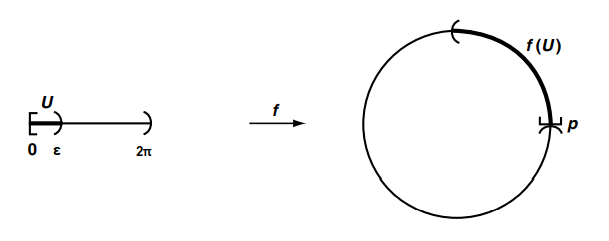
\includegraphics[scale = 0.6]{ex1.22}
\centering
\end{figure}
\end{example}

\begin{example}
Consideremos $B(0;1) \subset \R^n$ con $n \geq 1$ y veamos que $B(0;1) \cong \R^n$. Sea $f \colon B(0;1) \to \R^n$, $f(x) = \frac{x}{1-||x||}$. Nótese que $f$ está bien definida, pues si $x \in B(0;1)$, entonces $d(x,0) = ||x-0|| = ||x|| < 1$, luego $1-||x|| > 0$. Veamos que $f$ es homeomorfismo.
\begin{itemize}
    \item $f$ es continua por ser cociente de aplicaciones continuas.
    \item Describimos $f^{-1}$: sea $g \colon \R^n \to B(0;1)$, $g(y) = \frac{y}{1+||y||}$. Nótese que $g$ es continua por ser cociente de aplicaciones continuas y está bien definida, ya que $Im(g) \subset B(0;1)$: \[d(g(y),0) = ||g(y)|| = ||\frac{y}{1+||y||}|| = \frac{||y||}{1+||y||} < 1 \implies g(y) \in B(0;1) \ \forall \ y \in \R^n\]
    Hay que comprobar que $g \circ f = id_{B(0;1)}$ y que $f \circ g = id_{\R^n}$. Tenemos que \[g \circ f(x) = g(f(x)) = \frac{f(x)}{1+||f(x)||} = \frac{\frac{x}{1-||x||}}{1+\frac{||x||}{1-||x||}} = \frac{\frac{x}{1-||x||}}{\frac{1-||x||+||x||}{1-||x||}} = x\]
    La otra comprobación es similar. Por tanto, $g = f^{-1}$ y $f$ es también biyectiva.
\end{itemize}
\end{example}

\begin{example}
Sea $x_0 \in \R^n$ y sea $r > 0$. Veamos que $B(0;1) \cong B(x_0;r)$. Definimos $f \colon B(0;1) \to B(x_0;r)$, $f(x) = rx + x_0$. Nótese que si $x \in B(0;1)$ (por tanto $||x||<1$), entonces $f(x) \in B(x_0;r)$, pues \[d(f(x),x_0) = ||f(x) - x_0|| = ||rx|| = r||x|| < r\] Sea $g \colon B(x_0;r) \to B(0;1)$, $g(y) = \frac{y-x_0}{r}$ (que es continua). Nótese que si $y \in B(x_0;r)$, entonces $g(y) \in B(0;1)$, pues \[d(g(y),0) = ||g(y)|| = \frac{||y-x_0||}{r} = \frac{d(y,x_0)}{r} < \frac{r}{r} = 1\] Trivialmente, $g \circ f = id_{B(0;1)}$ y $f \circ g = id_{B(x_0;r)}$. Por tanto, $g = f^{-1}$ así que $f$ es homeomorfismo.
\end{example}

\begin{obs}
Como vimos que el carácter homeomorfo es una relación de equivalencia, de estos dos últimos ejemplos deducimos que $\R^n$ es homeomorfo a cualquiera de sus bolas abiertas.
\end{obs}

\begin{example}
\label{ex1.25.}
Consideremos $S^n = \{(x_1,\mathellipsis,x_{n+1}) \in \R^{n+1} \mid x_1^2 + \mathellipsis + x_{n+1}^2 = 1\} \subset \R^{n+1}$. Sea $N = \{(0,0,\mathellipsis,0,1)\} \subset \R^{n+1}$. Se comprueba que $S^n \setminus N \cong \R^n$ (Ejercicio 10 de la Relación 2).

\begin{figure}[h]
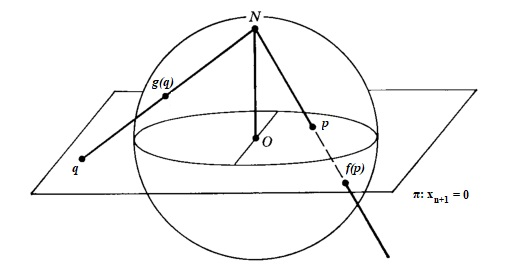
\includegraphics[scale = 0.8]{ex1.25}
\centering
\end{figure}

\end{example}

\section{Topología cociente}

Sea $X$ un espacio topológico y $\mathcal{R}$ una relación de equivalencia en $X$. Si pensamos en $\mathcal{R}$ como una \say{manipulación} del espacio $X$, queremos dotar al conjunto cociente $\faktor{X}{\mathcal{R}}$ de una topología que refleje tal \say{manipulación}. Observamos que dicha \say{manipulación} es la \underline{proyección canónica}: 
\[
\begin{aligned}[t]
    p \colon X & \longrightarrow \faktor{X}{\mathcal{R}} \\
    x & \longmapsto \overline{x}
\end{aligned}
\]

Vamos a dotar a $X$ de la mayor topología que haga que $p$ sea continua.

\begin{definition}
Un subconjunto $\theta \subset \faktor{X}{\mathcal{R}}$ de clases de equivalencia es \underline{abierto} si $p^{-1}(\theta)$ es abierto de $X$.
\end{definition}

\vspace{2mm}
En efecto, esto resulta ser una topología en $\faktor{X}{\mathcal{R}}$:
\begin{itemize}
    \item[(i)] Tanto $\emptyset$ como $\faktor{X}{\mathcal{R}}$ son abiertos.
    \item[(ii)] Si $\{\theta_i\}_{i \in I}$ es una familia de abiertos de $\faktor{X}{\mathcal{R}}$, entonces \[p^{-1}\biggl( \, \bigcup_{i \in I}\theta_i \biggr ) = \bigcup_{i \in I} \, p^{-1}(\theta_i)\]
    y como $\bigcup_{i \in I}p^{-1}(\theta_i)$ es abierto de $X$ por ser unión de abiertos de X, entonces $\bigcup_{i \in I}\theta_i$ es abierto de $\faktor{X}{\mathcal{R}}$.
    \item[(iii)] Análogo a (ii).
\end{itemize}

A esta topología se le denomina \underline{topología cociente}, y a $\faktor{X}{\mathcal{R}}$ \underline{espacio cociente}.

\vspace{2mm}
\begin{obs}
La topología cociente es la topología más grande que hace que la proyección canónica $p$ sea continua:
\begin{itemize}
    \item $p$ es continua con esta topología por definición.
    \item Sea $\tau$ otra topología que hace que $p$ sea continua y tomemos $\theta \in \tau$. Por la continuidad de $p$, se tiene que $p^{-1}(\theta)$ es abierto de $X$. Esto significa que $\theta$ es abierto de la topología cociente.
\end{itemize}
\end{obs}

\begin{proposition}
Sea $X$ un espacio topológico, $\mathcal{R}$ una relación de equivalencia en $X$ y $\faktor{X}{\mathcal{R}}$ el espacio cociente resultante. Una aplicación $f \colon \faktor{X}{\mathcal{R}} \to Y$ es continua si y solo si $f \circ p \colon X \to Y$ es continua.
\end{proposition}

\begin{proof}
\hfill
\begin{itemize}
    \item[{\fbox[rb]{$\Rightarrow$}}] Supongamos que $f \colon \faktor{X}{\mathcal{R}} \to Y$ es continua. Como hemos visto que $p \colon X \to \faktor{X}{\mathcal{R}}$ es continua, entonces $f \circ p \colon X \to Y$ es continua.
    \item[{\fbox[rb]{$\Leftarrow$}}] Supongamos que $f \circ p \colon X \to Y$ es continua. Tenemos que 
    \[
    \begin{aligned}[t]
        f \textrm{ es continua} &\iff f^{-1}(\theta) \textrm{ es abierto de } \faktor{X}{\mathcal{R}} \ \forall \ \theta \textrm{ abierto de } Y \\
        &\iff p^{-1}(f^{-1}(\theta)) \textrm{ es abierto de } X \ \forall \ \theta \textrm{ abierto de } Y \\
        &\iff (f \circ p)^{-1}(\theta) \textrm{ es abierto de } X \ \forall \ \theta \textrm{ abierto de } Y
    \end{aligned}
    \] Esto último es cierto porque $f \circ p$ es continua.
\end{itemize}
\end{proof}

\begin{obs}
Si $X$ es un espacio topológico y $A \subset X$, vamos a denotar por $\faktor{X}{A}$ al espacio cociente resultante de identificar todos los puntos de $A$ entre sí, es decir, $a \sim b$ si $a, b \in A$ y $x \sim x$ si $x \notin A$.
\end{obs}

\begin{example}
En $[0,1]$, consideramos la relación de equivalencia $0 \sim 1$, $1 \sim 0$ y $t \sim t$ si $t \in [0,1]$. Tomamos $\faktor{[0,1]}{\sim} = \faktor{[0,1]}{\{0,1\}}$. Veamos que $\faktor{[0,1]}{\sim} \cong S^1$. Definimos la aplicación $f \colon \faktor{[0,1]}{\sim} \to S^1$, $f(\overline{t}) = (\cos{2 \pi t}, \sen{2 \pi t})$. Tenemos que

\begin{itemize}
    \item $f$ está bien definida, pues si $t \sim t'$, puede ocurrir que
    \begin{itemize}
        \item $t = t' \implies f(\overline{t}) = f(\overline{t'})$
        \item $t = 0$ y $t' = 1$ (o viceversa) $\implies f(\overline{t}) = (1,0) = f(\overline{t'})$
    \end{itemize}
    \item $f$ es continua, pues la composición $f \circ p \colon [0,1] \to S^1, f(p(t)) = (\cos{2 \pi t}, \sen{2 \pi t})$ es claramente continua.
    \item $f$ es inyectiva, ya que si $f(\overline{t_1}) = f(\overline{t_2})$ con $t_1, t_2 \in [0,1]$, entonces
    \[
    \begin{cases}
        \cos{2 \pi t_1} = \cos{2 \pi t_2} \\
        \sen{2 \pi t_1} = \sen{2 \pi t_2}
    \end{cases} \implies t_1 - t_2 = k \in \Z \implies 
    \begin{cases}
        t_1 = t_2 \implies \overline{t_1} = \overline{t_2} \\
        t_1 = 0, t_2 = 1 \implies \overline{t_1} = \overline{t_2} \\
        t_1 = 1, t_2 = 0 \implies \overline{t_1} = \overline{t_2}
    \end{cases}
    \]
    En cualquier caso, $\overline{t_1} = \overline{t_2}$.
    \item $f$ es sobreyectiva, pues si $(x,y) \in S^1$ podemos escribir $x = \cos{2 \pi t}, y = \sen{2 \pi t}$ para algún $t \in [0,1]$, luego $(x,y) = f(\overline{t})$.
    \item $f$ es cerrada, pues $\faktor{[0,1]}{\sim}$ es compacto y $S^1$ es Hausdorff (\hyperref[cor3.4.]{\color{blue}Corolario 3.4}).
\end{itemize}

Por tanto, $f$ es homeomorfismo.

\begin{figure}[h]
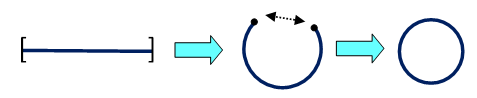
\includegraphics[scale = 0.7]{ex1.26}
\centering
\end{figure}

\end{example}

\begin{example}
Sean $X = [0,1] \times [0,1]$, $C = \{(x,y,z) \in \R^3 \mid x^2 + y^2 = 1, 0 \leq z \leq 1\}$. En $X$, consideramos la relación de equivalencia $(0,t) \sim (1,t) \ \forall \  t \in [0,1]$. Veamos que $\faktor{X}{\sim} \cong C$. Tomamos $f \colon \faktor{X}{\sim} \to C$, $f(\overline{s,t}) = (\cos{2 \pi s}, \sen{2 \pi s}, t)$. De forma similar al ejemplo anterior se comprueba que $f$ está bien definida y es continua, biyectiva y cerrada, por lo que $f$ es homeomorfismo.

\begin{figure}[h]
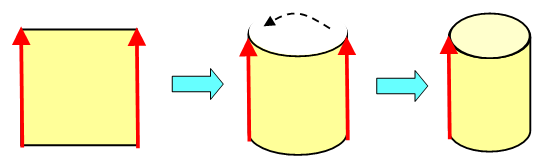
\includegraphics[scale = 0.7]{ex1.27}
\centering
\end{figure}

\end{example}

\section{Topología producto}

Sean $X, Y$ espacios topológicos. Queremos dotar a $X \times Y$ de una topología \say{compatible} con $X$ e $Y$.

\begin{definition}
La \underline{topología producto} en $X \times Y$ es la que tiene por base a \[\{U \times V \mid U \textrm{ abierto de } X \textrm{, } V \textrm{ abierto de } Y\}\] Esto significa que cualquier abierto $\theta$ de $X \times Y$ es de la forma \[\theta = \bigcup_{i \in I} \ (U_i \times V_i)\] con $U_i$ y $V_i$ abiertos de $X$ e $Y$ $\forall \ i \in I$. Por tanto, podemos escribir
\[\tau_{X \times Y} = \biggl\{ \, \bigcup_{i \in I} \ (U_i \times V_i) \mid U_i \textrm{ y } V_i \textrm{ abiertos de } X \textrm{ e } Y \ \forall \ i \in I \biggr\}\]
\end{definition}

\begin{proposition}
La topología en $X \times Y$ definida anteriormente es la menor topología en $X \times Y$ que hace que las proyecciones $p_X \colon X \times Y \to X$, $p_X(x,y) = x$ y $p_Y \colon X \times Y \to Y$, $p_Y(x,y) = y$ sean continuas.
\end{proposition}

\begin{proof}
\hfill
\begin{itemize}
    \item Veamos que $p_X \colon (X \times Y, \tau_{X \times Y}) \to X$ y $p_Y \colon (X \times Y, \tau_{X \times Y}) \to Y$ son continuas. Sean $U$ y $V$ abiertos de $X$ e $Y$, respectivamente. Entonces $p_X^{-1}(U) = U \times Y \in \tau_{X \times Y}$ y $p_Y^{-1}(V) = X \times V \in \tau_{X \times Y}$. Por tanto, $p_X$ y $p_Y$ son continuas.
    \item Sea $\tau$ otra topología en $X \times Y$ tal que $p_X \colon (X \times Y, \tau) \to X$, $p_Y \colon (X \times Y, \tau) \to Y$ son continuas. Veamos que $\tau_{X \times Y} \subset \tau$. Sean $\{U_i\}_{i \in I}$ y $\{V_i\}_{i \in I}$ familias de abiertos de $X$ e $Y$, respectivamente. Como $p_X^{-1}(U_i) = U_i \times Y \in \tau \ \forall \ i \in I$ y $p_Y^{-1}(V_i) = X \times V_i \in \tau \ \forall \ i \in I$ por ser $p_X,p_Y$ continuas, entonces $(U_i \times Y) \cap (X \times V_i) \in \tau \ \forall \ i \in I$. Además,
    \[(U_i \times Y) \cap (X \times V_i) = (U_i \cap X) \times (Y \cap V_i) = U_i \times V_i \in \tau \ \forall \ i \in I\]
    Por tanto,
    \[\bigcup_{i \in I} \ (U_i \times V_i) \in \tau \implies \tau_{X \times Y} \subset \tau\]
\end{itemize}
\end{proof}

\begin{obs}
Sean $(X, d_X), (Y, d_Y)$ espacios métricos. En $X \times Y$ podemos definir la \ul{distancia producto} como \[D \colon (X \times Y) \times (X \times Y) \to \R \textrm{, } D((x,y),(x',y')) = (d_X(x,x')^2 + d_Y(y,y')^2)^{\frac{1}{2}}\]
Se comprueba que la topología asociada a $(X \times Y, D)$ es, precisamente, la topología producto de $(X, d_X) \times (Y, d_Y)$. Por ejemplo, en $\R^2$, la distancia usual $d$ es la distancia producto de $(\R, | \ |) \times (\R, | \ |)$, ya que \[d((x,y),(x',y')) = ((x-x')^2+(y-y')^2)^\frac{1}{2}\] Se observa claramente que no todo abierto de la topología producto en $X \times Y$ es de la forma $U \times V$ con $U$ abierto de $X$ y $V$ abierto de Y, ya que $B(0;1) \subset \R^2$ es abierto de $\R^2$, pero no es de la forma $U \times V$ con $U, V$ abiertos de $\R$.
\end{obs}

\chapter{Conexidad}

\section{Introducción}

\begin{definition}
Un espacio topológico $X$ es \underline{conexo} si no puede escribirse como unión disjunta de dos abiertos no vacíos, es decir, si $X \neq \theta_1 \, \dot\cup \ \theta_2$ con $\theta_1, \theta_2$ abiertos no vacíos y tales que $\theta_1 \cap \, \theta_2 = \emptyset$.
\end{definition}

\begin{theorem}[Caracterización de los espacios conexos]
\label{teo2.1.}
Sea $X$ espacio topológico. Son equivalentes:
\begin{itemize}
    \item[(i)] $X$ es conexo.
    \item[(ii)] Los únicos abiertos y cerrados (simultáneamente) de $X$ son $\emptyset$ y $X$.
    \item[(iii)] No existe ninguna aplicación $f \colon X \to \{a,b\}$ con $\{a,b\}$ espacio discreto que sea continua y sobreyectiva.
\end{itemize}
\end{theorem}

\begin{proof}
Veamos primero que $(i) \iff (ii)$.
\begin{itemize}
    \item[{\fbox[rb]{$\Rightarrow$}}] Supongamos que $A \subset X$ con $A \neq X$ y $A \neq \emptyset$ es abierto y cerrado. Entonces tenemos que $X = A \ \dot\cup \ A^c$, luego $X$ no es conexo.
    \item[{\fbox[rb]{$\Leftarrow$}}] Supongamos que $X$ no es conexo. Esto significa que $X = \theta_1 \, \dot\cup \ \theta_2$ con $\theta_1, \theta_2$ abiertos no vacíos y tales que $\theta_1 \cap \, \theta_2 = \emptyset$. Por tanto, $\theta_1 = \theta_2^c$ es cerrado, así que $\theta_1$ es abierto y cerrado distinto de $X$ y de $\emptyset$.
\end{itemize}

\vspace{2mm}
Veamos ahora que $(i) \iff (iii)$.
\begin{itemize}
    \item[{\fbox[rb]{$\Rightarrow$}}] Supongamos que $f \colon X \to \{a,b\}$ es continua y sobreyectiva con $\{a,b\}$ espacio discreto. Entonces $X = f^{-1}(\{a\}) \cup f^{-1}(\{b\})$ con ambos abiertos (en la topología discreta todo subconjunto es abierto) y no vacíos ($f$ es sobreyectiva). Por tanto, $X$ no es conexo.
    \item[{\fbox[rb]{$\Leftarrow$}}] Supongamos que $X$ no es conexo, es decir, $X = \theta_1 \, \dot\cup \ \theta_2$ con $\theta_1, \theta_2$ abiertos no vacíos y tales que $\theta_1 \cap \, \theta_2 = \emptyset$. Entonces la aplicación $f \colon X \to \{a,b\}$ definida por
    \[
    f(x) =
    \begin{cases}
        a & $si$ \ x \in \theta_1 \\
        b & $si$ \ x \in \theta_2
    \end{cases}
    \]
    para cualquier espacio discreto $\{a,b\}$ es sobreyectiva ($\theta_1, \theta_2 \neq \emptyset$) y continua, ya que \[f^{-1}(\emptyset) = \emptyset, f^{-1}(\{a\}) = \theta_1, f^{-1}(\{b\}) = \theta_2, f^{-1}(\{a,b\}) = X\]
\end{itemize}
\end{proof}

\begin{obs}
Si $Y \subset X$ con $X$ espacio topológico, en adelante, para ahorrar escritura, diremos simplemente que $Y$ es (o no) conexo. La conexidad es una característica propia de los espacios topológicos, así que lo que estamos diciendo en realidad es que el subconjunto $Y$ con la topología de subespacio es (o no) un espacio conexo.
\end{obs}

\begin{example}
Sea $X$ un espacio discreto de más de un punto. Entonces $X$ no es conexo, pues cualquier subconjunto de $X$ es abierto y cerrado.
\end{example}

\begin{example}
Todo espacio grosero es conexo.
\end{example}

\begin{example}
Sea $X$ un conjunto infinito dotado de la topología de los complementos finitos (\hyperref[ex1.5.]{\color{blue}Ejemplo 1.5}). Entonces $X$ es conexo, pues si $\emptyset \subsetneq A \subsetneq X$ es cerrado y abierto, entonces $A^c$ es finito por ser $A$ abierto y $A$ es también finito por ser $A$ cerrado. Por tanto, $X = A \cup A^c$ tendría que ser finito, que es una contradicción.
\end{example}

\begin{example}
Sea $X$ un espacio dotado de la topología del punto excluido (ver Relación 1). Entonces $X$ es conexo, pues si $\emptyset \subsetneq A \subsetneq X$ es cerrado y abierto, entonces $x_0 \in A$ y $x_0 \notin A$, lo cual es imposible.
\end{example}

\begin{example}
$\Q \subset \R$ no es conexo, ya que si tomamos $x \in \R \setminus \Q$, podemos escribir $\Q$ como unión de abiertos disjuntos y no vacíos: \[\Q = ((-\infty,x) \cap \Q) \ \dot\cup \ ((x,\infty) \cap \Q)\] De igual forma se comprueba que $\R \setminus \Q$ no es conexo.
\end{example}

\begin{example}
En $\R^3$, consideramos $X = \overline{B}(0;1) \ \dot\cup \ \{(0,2,0)\}$. Entonces $X$ no es conexo.
\end{example}

\begin{example}
En $\R^2$, consideramos $X = B(0;1) \ \dot\cup \ B((2,0);1)$. Entonces $X$ no es conexo.
\end{example}

\section{Propiedades de la conexidad}

\begin{proposition}
\label{prop2.1.}
Sea $X$ un espacio topológico y $B \subset X$ conexo. Entonces $\overline{B}$ es conexo.
\end{proposition}

\begin{proof}
Supongamos que $\overline{B}$ no es conexo. Entonces existe $f \colon \overline{B} \to \{a,b\}$ continua y sobreyectiva, con $\{a,b\}$ espacio discreto. Es claro que $f(B) \subset \{a,b\}$ y también tenemos que $f(B) \supset \{a,b\}$, ya que
\[\{a,b\} = f(\overline{B}) \subset \overline{f(B)} = f(B)\]
En la primera igualdad hemos usado que $f$ es sobreyectiva, en la contención el Ejercicio 1 de la Relación 2 y en la segunda igualdad que $f(B)$ es cerrado del espacio discreto $\{a,b\}$. Por tanto, la restricción de $f$ a $B$, $\left.f\right|_B \colon B \to \{a,b\}$, es también continua (\hyperref[prop1.15.]{\color{blue}Proposición 1.15}) y sobreyectiva (porque $f(B) = \{a,b\}$), lo que significa que $B$ no es conexo. 
\end{proof}

\begin{proposition}
Sea $X$ un espacio topológico y $\{A_i\}_{i \in I}$ una familia de subespacios conexos de $X$ tales que $A_i \cap A_j \neq \emptyset \ \forall \ i,j \in I$. Entonces $\bigcup_{i \in I}A_i$ es conexo.
\end{proposition}

\begin{proof}
Sea $f \colon \bigcup_{i \in I}A_i \to \{a,b\}$ continua con $\{a,b\}$ espacio discreto y veamos que $f$ no puede ser sobreyectiva, es decir, es necesariamente constante. Sean $x,y \in \bigcup_{i \in I}A_i$. Entonces $x \in A_j$, $y \in A_k$ para ciertos $j,k \in I$. Puesto que $A_j \cap A_k \neq \emptyset$, podemos tomar $z \in A_j \cap A_k$. Consideremos $\left.f\right|_{A_j} \colon A_j \to \{a,b\}$, que es continua. Como $A_j$ es conexo, $\left.f\right|_{A_j}$ no puede ser sobreyectiva, es decir, debe ser constante, por lo que $f(x) = f(z)$. Repetimos el mismo razonamiento con $A_k$ y tenemos que $f(y) = f(z) = f(x)$, por lo que $f$ es constante y $\bigcup_{i \in I}A_i$ es conexo. 
\end{proof}

\begin{proposition}
Sean $X,Y$ espacios topológicos y sea $f \colon X \to Y$ continua. Si $X$ es conexo, entonces $Im(f)$ es un subespacio conexo de $Y$.
\end{proposition}

\begin{proof}
Por reducción al absurdo, supongamos que $Im(f)$ no es conexo. Entonces existe $g \colon Im(f) \to \{a,b\}$ continua y sobreyectiva con $\{a,b\}$ espacio discreto. Por tanto, la composición $g \circ f \colon X \to \{a,b\}$ es continua y sobreyectiva. Esto significa que $X$ no es conexo, lo que contradice la hipótesis.
\end{proof}

\begin{obs}
Si $f \colon X \to Y$ es continua y $X$ es conexo, $Y$ no tiene por qué ser conexo. Por ejemplo, si tomamos $f \colon (0,1) \to (0,1) \ \dot\cup \ (4,5), f(x) = x$, tenemos que $X$ es conexo ($Im(f)$ también), pero $Y$ no lo es.
\end{obs}

\vspace{1mm}
El siguiente teorema nos dice que un espacio topológico homeomorfo a un espacio conexo es también conexo. En general, se dice que una propiedad $p$ es un \underline{invariante topológico} si es invariante por homeomorfismos, esto es, si $X$ verifica $p$ y $X \cong Y$, entonces $Y$ verifica $p$.

\begin{theorem}
La conexidad es un invariante topológico.
\end{theorem}

\begin{proof}
Sea $X$ un espacio topológico conexo y supongamos que $X \cong Y$ mediante un homeomorfismo $f \colon X \xrightarrow{\cong} Y$. Como $f$ es sobreyectiva, entonces $Im(f) = Y$, y como $f$ es continua, por la prosición anterior, tenemos que $Y$ es conexo.
\end{proof}

\section{Conexidad de los subespacios de $\R$}

\begin{theorem}
$[a,b]$ es conexo.
\end{theorem}

\begin{proof}
Supongamos que $[a,b]$ no es conexo, es decir, $[a,b] = U \ \dot\cup \ V$ con $U,V$ abiertos de $[a,b]$ disjuntos y no vacíos. Supongamos, sin pérdida de generalidad, que $a \in U$. Por ser $U$ abierto, para cierto $\varepsilon > 0$ se tiene que $[a,\varepsilon) \subset U$. Sea $B = \{t \in [a,b] \mid  t < v \ \forall \ v \in V\}$. Tenemos que $B \subset U$, $B \neq \emptyset$ (ya que $[a,\varepsilon) \subset B$) y $B$ está acotado superiormente, por lo que tiene supremo $t_0$. Nótese que $t_0 < b$, pues si fuese $t_0 = b$, tendríamos que $U = [a,b]$ y $V = \{b\}$, que no es abierto. Tomemos $(t_0 - \delta, t_0 + \delta) \subset [a,b]$ para cierto $\delta > 0$. Entonces $(t_0 - \delta, t_0 + \delta) \cap U \neq \emptyset$, pues $t_0$ es el supremo de $B$. Por tanto, $t_0 \in \overline{U} = U$ (ya que $U$ es abierto y cerrado de $[a,b]$), pero, por otra parte, $(t_0 - \delta, t_0 + \delta) \cap V \neq \emptyset$, porque en otro caso tendríamos que $[a,t_0+\delta) \subset U$ y esto contradiría que $t_0 = \sup{U}$. Por tanto, $t_0 \in \overline{V} = V$ y $t_0 \in U \cap V = \emptyset$. Esto es una contradicción, así que $[a,b]$ es conexo.
\end{proof}

\begin{corollary}
Los únicos subespacios conexos de $\R$ son los intervalos: 
\[\R, [a,b), (a,b], [a,b], (a,b), (-\infty,a), (-\infty,a], (a,\infty), [a,\infty)\]
\end{corollary}

\begin{proof}
Cualquier intervalo puede escribirse como unión de intervalos cerrados de intersección no vacía. Por ejemplo, \[(a,b) = \bigcup_{n=1}^{\infty} \, [a+\frac{1}{n},b+\frac{1}{n}]\] Por el teorema anterior, como los intervalos cerrados son conexos, concluimos que todos los intervalos son conexos. Por último, sea $X \subset \R$ no intervalo y veamos que $X$ no es conexo. Como $X$ no es un intervalo, existen $x_0 < y < x_1$ con $x_0,x_1 \in X, y \notin X$. Teniendo en cuenta que $x_0 \in X \cap (-\infty,y)$, $x_1 \in X \cap (y,\infty)$, podemos escribir $X$ como unión disjunta de abiertos no vacíos: \[X = (X \cap (-\infty,y)) \ \dot\cup \ (X \cap (y,\infty))\] Por tanto, $X$ no es conexo.
\end{proof}

\begin{theorem}[Teorema de los valores intermedios]
Sea $f \colon X \to \R$ continua con $X$ conexo. Si $f(x_0) = a, f(x_1) = b$, con $x_0, x_1 \in X$ y $a < b$, entonces para todo $c \in [a,b]$ existe $y \in X$ tal que $f(y) = c$. 
\end{theorem}

\begin{proof}
En las condiciones del enunciado, tenemos que $f(X)$ es un subespacio conexo de $\R$, es decir, $f(X)$ es un intervalo con $a,b \in f(X)$. Por tanto, $[a,b] \subset f(X)$.
\end{proof}

\begin{corollary}[Teorema de Bolzano]
Sea $f \colon X \to \R$ continua con $X$ conexo. Supongamos que $f(x_0) < 0$ y $f(x_1) > 0$ para ciertos $x_0,x_1 \in X$. Entonces existe $y \in X$ tal que $f(y) = 0$.
\end{corollary}

\section{Componentes conexas de un espacio topológico}

Sea $X$ un espacio topológico. Vamos a establecer en $X$ la siguiente relación: $x \sim y$ si existe $C \subset X$ conexo tal que $x,y \in C$. Comprobemos, en primer lugar, que esta relación es de equivalencia:
\begin{itemize}
    \item $x \sim x$ porque $\{x\}$ es conexo.
    \item La relación es simétrica por definición.
    \item Supongamos que $x \sim y$, $y \sim z$. Entonces existe $C \subset X$ conexo tal que $x,y \in C$ y existe $D \subset X$ conexo tal que $y,z \in D$. Por tanto, $x,z \in C \cup D$, que es conexo por ser unión de conexos con intersección no vacía ($y \in C \cap D)$, así que $x \sim z$.
\end{itemize}

A cada clase de equivalencia la llamamos \underline{componente conexa}. Denotamos por $C(x)$ a la componente conexa del punto $x \in X$.

\begin{proposition}
\label{prop2.4.}
Sea $X$ un espacio topológico. La componente conexa de un punto $x \in X$ es el mayor subespacio conexo de $X$ que contiene a $x$.
\end{proposition}

\begin{proof}
\hfill
\begin{itemize}
    \item Veamos que $C(x)$ es un subespacio conexo. Para cada $y \in C(x)$, existe un conexo $D_y$ tal que $x,y \in D_y$. Comprobemos que $C(x) = \bigcup_{y \in C(x)}D_y$:
    \begin{itemize}
        \item[{\fbox[rb]{$\subset$}}] Elemental.
        \item[{\fbox[rb]{$\supset$}}] Sea $z \in \bigcup_{y \in C(x)}D_y$. Entonces $z \in D_{y_0}$ para algún $y_0 \in C(x)$, y como $D_{y_0}$ es conexo, $z \sim y_0 \sim x$, luego $z \in C(x)$.
    \end{itemize}
    Tenemos que $C(x)$ es conexo por ser unión de conexos con intersecciones dos a dos no vacías ($x \in D_y \ \forall \ y \in C(x)$).
    \item Veamos que $C(x)$ es el mayor conexo que contiene a $x$. Supongamos que $C$ es conexo con $C \supsetneq C(x)$. Entonces existe $y \in C$ con $y \notin C(x)$. Tenemos que $y \nsim x$, pero $x,y \in C$ y $C$ es conexo, así que $y \sim x$, que es una contradicción.
\end{itemize}
\end{proof}

\begin{corollary}
Sea $X$ un espacio topológico y sea $x \in X$. Entonces \[C(x) = \bigcup_{\substack{C \, \emph{con.} \\ x \in C}}C\]
\end{corollary}

\begin{obs}
$C(x) = C(y) \ \forall \ y \in C(x)$, ya que $\overline{x} = \overline{y} \iff x \sim y$.
\end{obs}

\begin{proposition}
\label{prop2.5.}
El conjunto de componentes conexas constituye una partición en $X$ por subespacios conexos y cerrados de $X$.
\end{proposition}

\begin{proof}
Es obvio que el conjunto de componentes conexas constituye una partición en $X$ y que todas con conexas. Veamos que son cerradas. Sea $C$ una componente conexa y veamos que $C = \overline{C}$. Sabemos que $C \subset \overline{C}$ y $\overline{C}$ es conexo, así que tiene que ser $C = \overline{C}$ porque $C$ es el mayor conexo que contiene a cualquiera de sus puntos.
\end{proof}

\begin{obs}
\hfill
\begin{itemize}
    \item En general, las componentes conexas no son abiertos.
    \item Se tiene que $X$ es conexo si y solo si $X$ solo tiene una componente conexa.
\end{itemize}
\end{obs}

\begin{example}
Sea $X = (0,1) \cup (2,3) \cup (4,6)$. Veamos que las componentes conexas de $X$ son $(0,1)$, $(2,3)$ y $(4,6)$. Tenemos que $(0,1)$ es conexo por ser un intervalo. Si existiera $C \subset X$ conexo con $C \supsetneq (0,1)$, existiría $x_0 \in C$ con $x_0 \notin (0,1)$, por lo que $C$ tendría que contener un intervalo que contenga a $(0,1)$ y a $x_0 \in (2,3) \cup (4,6)$, lo cual es imposible. Con el mismo argumento se prueba que $(2,3)$ y $(4,6)$ son componentes conexas de $X$.
\end{example}

\begin{example}
Sea $x \in \Q$. Entonces $C(x)$ ha de ser un intervalo que solo contenga a $x$ y a números racionales, por lo que solo puede ser $C(x) = [x,x] = \{x\}$. Como las componentes conexas de $\Q$ se reducen a los puntos de $\Q$, decimos que $\Q$ es \underline{totalmente disconexo}. $\Q$ tiene una cantidad numerable de componentes conexas y ninguna de ellas es un abierto.
\end{example}

\begin{example}
Sea $X$ un espacio discreto y sea $x \in X$. Entonces $C(x) = \{x\}$, pues $\{x\}$ es conexo y si tomamos $Y \supsetneq \{x\}$ podemos escribir $Y = \{x\} \ \dot\cup \ (Y \setminus \{x\})$. Como $\{x\}$ y $Y \setminus \{x\}$ son abiertos no vacíos, tenemos que $Y$ no es conexo.
\end{example}

\vspace{2mm}
\begin{theorem}
\label{teo2.5.}
El cardinal del conjunto de componentes conexas de un espacio topológico es un invariante topológico.
\end{theorem}

\begin{proof}
Denotamos $C(X)$ al conjunto de componentes conexas de $X$. Consideremos un homeomorfismo $f \colon X \to Y$. Vamos a construir una biyección $C(f) \colon C(X) \to C(Y)$. Sea $C \in C(X)$ una componente conexa de $X$. Como $f$ es continua y $C$ es conexo, entonces $f(C) \subset Y$ es conexo. Además, $f(C)$ ha de estar contenido en una componente conexa $D$ de $Y$. Definimos $C(f)(C) = D$. Veamos que $C(f) \colon C(X) \to C(Y)$ es biyectiva comprobando que tiene inversa $C(f^{-1}) \colon C(Y) \to C(X)$. Tomamos $f^{-1} \colon Y \to X$, que es continua, así que podemos definir $C(f^{-1})$ como antes. Veamos que $C(f^{-1}) \circ C(f) = id_{C(X)}$. Sea $C \in C(X)$. Entonces
\[C(f^{-1}) \circ C(f)(C) = C(f^{-1})(C(f)(C)) = C(f^{-1})(D)\]
donde $D$ es la única componente conexa de $Y$ con $f(C) \subset D$. Por otra parte,
\[f^{-1}(D) \supset f^{-1}(f(C)) = C\]
Como $f^{-1}(D)$ es un conexo de $X$ que contiene a la componente conexa $C$, deben ser iguales. Tenemos entonces que $f^{-1}(D) = C$ está contenido en la componente conexa $C$ de $X$. Por definición de $C(f^{-1})$, esto significa que $C(f^{-1})(D) = C = C(f^{-1}) \circ C(f)(C)$. Análogamente se comprueba que $C(f) \circ C(f^{-1}) = id_{C(Y)}$, por lo que $C(f^{-1})$ es la inversa de $C(f)$ y $C(f)$ es biyectiva.
\end{proof}

\section{Arcoconexidad}

\begin{definition}
Una \underline{curva} en un espacio topológico $X$ es una aplicación $\alpha \colon [0,1] \to X$ continua.
\end{definition}

\vspace{2mm}
Dada una curva $\alpha \colon [0,1] \to X$, podemos definir una nueva curva $\alpha^{-1} \colon [0,1] \to X$ por $\alpha^{-1}(t) = \alpha(1-t)$. Nótese que $\alpha^{-1}$ es continua, pues la composición 
\[
\begin{aligned}[t]
    [0,1] & \xlongrightarrow{\cong} [0,1] \, \xlongrightarrow{\alpha} X \\
    t     & \longmapsto 1-t \longmapsto \alpha(1-t)
\end{aligned}
\] 
es continua. Se cumple que $Im(\alpha) = Im(\alpha^{-1})$ pero $\alpha \neq \alpha^{-1}$. Además, $\alpha^{-1}(0) = \alpha(1)$ y $\alpha^{-1}(1) = \alpha(0)$.

\vspace{2mm}
Sean $\alpha, \beta \colon [0,1] \to X$ curvas en $X$ con $\alpha(1) = \beta(0)$. Definimos una nueva curva 
\[
\alpha\beta \colon [0,1] \to X, \ \alpha\beta(t) = \begin{cases}
    \alpha(2t)  & $si$ \ 0 \leq t \leq \frac{1}{2} \\ 
    \beta(2t-1) & $si$ \ \frac{1}{2} \leq t \leq 1
\end{cases}
\]
Veamos que $\alpha\beta$ es, en efecto, continua:
\begin{itemize}
    \item $\alpha\beta$ está definida en dos cerrados, $[0, \frac{1}{2}]$ y $[\frac{1}{2},1]$, con $[0, \frac{1}{2}] \cup [\frac{1}{2},1] = [0,1]$.
    \item En cada uno de los cerrados, $\alpha\beta$ es continua por ser composición de funciones continuas.
    \item En la intersección de los cerrados, tenemos $\alpha\beta(\frac{1}{2}) = \alpha(2\frac{1}{2}) = \alpha(1) = \beta(0) = \beta(2\frac{1}{2}-1)$.
\end{itemize}

Por la \hyperref[prop1.16.]{\color{blue}Proposición 1.16}, $\alpha\beta$ es continua.

\begin{figure}[h]
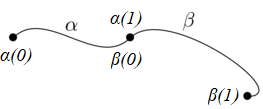
\includegraphics[scale = 1.0]{def2.2}
\centering
\end{figure}

\vspace{2mm}
\begin{definition}
Un espacio topológico $X$ es \underline{arcoconexo} si dos puntos cualesquiera de $X$ pueden unirse por una curva, es decir, si dados $x,y \in X$, existe una curva $\alpha \colon [0,1] \to X$ tal que $\alpha(0) = x, \alpha(1) = y$.
\end{definition}

\begin{theorem}[Caracterización de la arcoconexidad]
\label{teo2.6.}
Sea $X$ un espacio topológico y sea $x_0 \in X$. Son equivalentes:
\begin{itemize}
    \item[(i)] $X$ es arcoconexo.
    \item[(ii)] Todo punto de $X$ se une con $x_0$ por una curva, es decir, dado $y \in X$, existe una curva $\alpha \colon [0,1] \to X$ tal que $\alpha(0) = x_0$, $\alpha(1) = y$.
\end{itemize}
\end{theorem}

\begin{proof}
\hfill
\begin{itemize}
    \item[{\fbox[rb]{$\Rightarrow$}}] Es evidente.
    \item[{\fbox[rb]{$\Leftarrow$}}] Sean $y,z \in X$. Hay que encontrar una curva que una $y$ con $z$. Por hipótesis, existen curvas $\alpha_y, \alpha_z \colon [0,1] \to X$ con $\alpha_y(0) = x_0, \alpha_y(1) = y, \alpha_z(0) = x_0, \alpha_z(1) = z$. Nótese que $\alpha_y^{-1}(1) = \alpha_y(0) = x_0 = \alpha_z(0)$ y tiene sentido, por tanto, la curva $\alpha_y^{-1}\alpha_z \colon [0,1] \to X$. Además, 
    \begin{itemize}
        \item $\alpha_y^{-1}\alpha_z(0) = \alpha_y^{-1}(2 \cdot 0) = \alpha_y^{-1}(0) = \alpha_y(1) = y$
        \item $\alpha_y^{-1}\alpha_z(1) = \alpha_z(2 \cdot 1 - 1) = \alpha_z(1) = z$
    \end{itemize}
    Por tanto, $X$ es arcoconexo.
\end{itemize}
\end{proof}

\vspace{2mm}
Para los ejemplos que siguen, serán necesarias las siguientes definiciones:

\begin{definition}
Un subconjunto $X \subset \R^n$ es \underline{convexo} si dados dados $x_0,x_1 \in X$, se verifica que $\overline{x_0x_1} = \{(1-t)x_0 + tx_1 \mid t \in [0,1]\} \subset X$.
\end{definition}

\begin{definition}
Un subconjunto $X \subset \R^n$ es \underline{estrellado respecto de $x_0 \in X$} si dado $x \in X$ se verifica que $\overline{x_0x} = \{(1-t)x_0 + tx \mid t \in [0,1]\} \subset X$.
\end{definition}

\vspace{2mm}
\begin{example}
Si $X \subset \R^n$ es un subespacio convexo, entonces es arcoconexo. En efecto, dados $x,y \in X$, tomamos la curva $\alpha \colon [0,1] \to X$, $\alpha(t) = (1-t)x + ty$, que es continua y está bien definida por ser $X$ convexo. Tenemos que $\alpha(0) = x$ y $\alpha(1) = y$, así que $X$ es arcoconexo.
\end{example}

\begin{example}
Si $X \subset \R^n$ es un subespacio estrellado respecto de $x_0 \in X$, entonces es arcoconexo. En efecto, usando el \hyperref[teo2.6.]{\color{blue}Teorema 2.6}, si tomamos $x \in X$, la curva $\alpha \colon [0,1] \to X$, $\alpha(t) = (1-t)x_0 + tx$ está bien definida (por ser $X$ estrellado respecto de $x_0$) y además cumple $\alpha(0) = x_0$, $\alpha(1) = x$. Por tanto, $X$ es arcoconexo.
\end{example}

\vspace{2mm}
\begin{theorem}
Todo espacio arcoconexo es conexo.
\end{theorem}
\begin{proof}
Sea $X$ un espacio topológico arcoconexo. Por reducción al absurdo, supongamos que $X$ no es conexo. Entonces existe $f \colon X \to \{a,b\}$ continua y sobreyectiva con $\{a,b\}$ espacio discreto. Sean $x_0, x_1 \in X$ tales que $f(x_0) = a, f(x_1) = b$. Por ser $X$ arcoconexo, existe una curva $\alpha \colon [0,1] \to X$ tal que $\alpha(0) = x_0$, $\alpha(1) = x_1$. Consideremos la composición $f \circ \alpha \colon [0,1] \to \{a,b\}$, que es continua y sobreyectiva (ya que $f \circ \alpha(0) = a, f \circ \alpha(1) = b$). Esto significa que $[0,1]$ no es conexo, que es imposible.
\end{proof}

\begin{corollary}
$\R^n$ y cualquier bola (abierta o cerrada) de $\R^n$ son espacios conexos.
\end{corollary}

\begin{obs}
En general, el recíproco del teorema anterior no es cierto, como se comprueba en el siguiente ejemplo:
\end{obs}

\begin{example}
Sea $f \colon (0,1] \to \R$, $f(x) = \sen{(\frac{1}{x})}$. Definimos 
\[X = gr\acute{a}f(f) \cup (\{0\} \times [-1,1]) \subset \R^2\]
Tenemos que $gr\acute{a}f(f) \cong \R \cong (0,1]$ (para el primer homeomorfismo, ver el Ejercicio 9 de la Relación 2) y $(0,1]$ es conexo, así que $gr\acute{a}f(f)$ también lo es. Por tanto, $\overline{gr\acute{a}f(f)} = X$ es conexo. Sin embargo, $X$ no es arcoconexo (Ejercicio 8 de la Relación 4).

\begin{figure}[h]
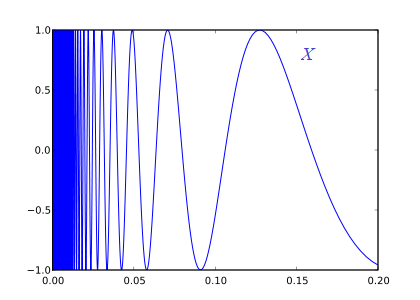
\includegraphics[scale = 0.8]{ex2.13}
\centering
\end{figure}

No obstante...
\end{example}

\begin{obs}
Sea $X \subset \R$. $X$ es conexo $\iff$ $X$ es arcoconexo $\iff$ $X$ es un intervalo.
\end{obs}

\vspace{2mm}
En el ejemplo anterior hemos usado que si $A \subset X$ es conexo entonces $\overline{A}$ es también conexo (\hyperref[prop2.1.]{\color{blue}Proposición 2.1}). Sin embargo, existen subespacios $A \subset X$ arcoconexos tales que $\overline{A}$ no es arcoconexo. Por ejemplo, en el conjunto $X$ del ejemplo de antes, tomamos $A = gr\acute{a}f(f) \subset X$. Tenemos que $A$ es arcoconexo (pues es homeomorfo a $(0,1]$) pero $\overline{A} = X$ no lo es.

\begin{proposition}
Sea $X$ un espacio topológico y sea $\{A_i\}_{i \in I}$ una familia de subespacios arcoconexos de $X$ tales que $A_j \cap A_k \neq \emptyset \ \forall \ j,k \in I, j \neq k$. Entonces $\bigcup_{i \in I}A_i$ es un subespacio arcoconexo de $X$. 
\end{proposition}

\begin{proof}
Sean $x,y \in \bigcup_{i \in I}A_i$. Entonces $x \in A_j, y \in A_k$ para ciertos $j,k \in I$. Tomemos $z \in A_j \, \cap \, A_k$. Como $A_j$ es arcoconexo, existe una curva $\alpha \colon [0,1] \to A_j$ con $\alpha(0) = x, \alpha(1) = z$, y como $A_k$ es arcoconexo, existe una curva $\beta \colon [0,1] \to A_k$ tal que $\beta(0) = z, \beta(1) = y$. Tomamos la curva $\alpha\beta \colon [0,1] \to \bigcup_{i \in I}A_i$, que está bien definida porque $\alpha(1) = \beta(0) = z$, y cumple que $\alpha\beta (0) = \alpha(0) = x, \alpha\beta(1) = \beta(1) = y$. Por tanto, $\bigcup_{i \in I}A_i$ es arcoconexo.
\end{proof}

\begin{proposition}
Sea $f \colon X \to Y$ continua con $X$ arcoconexo. Entonces $Im(f) = f(X)$ es un subespacio arcoconexo de $Y$.
\end{proposition}

\begin{proof}
Sean $y_0, y_1 \in Im(f)$. Entonces $y_0 = f(x_0)$, $y_1 = f(x_1)$ para ciertos $x_0,x_1 \in X$. Como $X$ es arcoconexo, existe una curva $\alpha \colon [0,1] \to X$ con $\alpha(0) = x_0, \alpha(1) = x_1$. Entonces la composición $f \circ \alpha \colon [0,1] \to Im(f)$ es una curva en $Im(f)$ con $f \circ \alpha(0) = y_0, f \circ \alpha(1) = y_1$, luego $Im(f)$ es arcoconexo.
\end{proof}

\begin{corollary}
La arcoconexidad es un invariante topológico.
\end{corollary}

\begin{proof}
Supongamos que $X$ es un espacio arcoconexo homeomorfo a $Y$ mediante un homeomorfismo $f \colon X \xrightarrow{\cong} Y$. Por la proposición anterior, $Im(f) = Y$ es arcoconexo.
\end{proof}

\begin{corollary}
$\R^n$ $(n>1)$ no es homeomorfo a $\R$.
\end{corollary}

\begin{proof}
Por reducción al absurdo, supongamos que $\R^n \cong \R$ y tomemos un homeomorfismo $f \colon \R^n \to \R$. Entonces, si $x_0 \in \R^n$, $\left.f\right|_{\R^n \setminus \{x_0\}} \colon \R^n \setminus \{x_0\} \to \R \setminus \{f(x_0)\}$ es también homeomorfismo, con inversa $\left.f^{-1}\right|_{\R^n \setminus \{x_0\}}$. Tenemos que $\R^n \setminus \{x_0\}$ es arcoconexo (Ejercicio 5 de la Relación 4) pero $\R \setminus \{f(x_0)\}$ no lo es (pues no es conexo), así que es imposible que sean homeomorfos.
\end{proof}

\begin{corollary}
\label{cor2.7.}
Sea $X$ un espacio topológico arcoconexo y $\sim$ una relación de equivalencia en $X$. Entonces $\faktor{X}{\sim}$ es arcoconexo.
\end{corollary}

\begin{proof}
Recordemos que la proyección canónica
\[
\begin{aligned}[t]
    p \colon X & \longrightarrow \faktor{X}{\sim} \\
    x & \longmapsto \overline{x}
\end{aligned}
\]
es continua y sobreyectiva, luego $Im(f) = \faktor{X}{\sim}$ es arcoconexo por serlo $X$.
\end{proof}

\begin{obs}
En particular, todo espacio cociente $\faktor{X}{\sim}$ con $X = [0,1] \times [0,1]$ es arcoconexo (banda de Moebius, toro, $S^2$, botella de Klein...).
\end{obs}

\section{Componentes arcoconexas}

Sea $X$ un espacio topológico. Definimos en $X$ la siguiente relación: $x \sim y$ si existe un subespacio arcoconexo $C \subset X$ tal que $x,y \in C$. Esta relación es de equivalencia y la comprobación es totalmente análoga a la que se hizo en la sección de las componentes conexas. A cada clase de equivalencia de esta relación la llamamos \underline{componente arcoconexa}.

\begin{proposition}
Sea $X$ un espacio topológico. La componente arcoconexa de un punto $x \in X$ es el mayor subespacio arcoconexo de $X$ que contiene a $x$.
\end{proposition}

\begin{proof}
Totalmente análoga a la de la \hyperref[prop2.4.]{\color{blue}Proposición 2.4}.
\end{proof}

\begin{corollary}
Sea $X$ un espacio topológico y sea $x \in X$. Entonces, si llamamos $C(x)$ a la componente arcoconexa que contiene a $x$, se tiene que \[C(x) = \bigcup_{\substack{C \, \emph{arcoc.} \\ x \in C}}C\]
\end{corollary}

\begin{obs}
El conjunto de componentes arcoconexas de $X$ constituye una partición de $X$ por subespacios arcoconexos. Sin embargo, como veremos en el ejemplo siguiente, las componentes arcoconexas, en general, no son cerrados de $X$, al contrario de las componentes conexas (\hyperref[prop2.5.]{\color{blue}Proposición 2.5}).
\end{obs}

\begin{example}
Sea $f \colon (0,1] \to \R$, $f(x) = \sen{(\frac{1}{x})}$. Definimos 
\[X = gr\acute{a}f(f) \cup (\{0\} \times [-1,1]) \subset \R^2\]
Las componentes arcoconexas de $X$ son $C_1 = gr\acute{a}f(f)$ y $C_2 = \{0\} \times [-1,1]$, ya que
\begin{itemize}
    \item $C_1$ es homeomorfo a $gr\acute{a}f(f) \cong (0,1]$ y es, por tanto, arcoconexo. Además, si tenemos que $C_1 \subsetneq A \subset X$, entonces $A$ no es arcoconexo.
    \item $C_2$ es homeomorfo a $[-1,1]$ y es, por tanto, arcoconexo. Igual que antes, si $C_2 \subsetneq B \subset X$, entonces $B$ no es arcoconexo.
\end{itemize}
Sin embargo, $C_1$ no es cerrado de $X$, pues $\overline{C_1} = X \neq C_1$.
\end{example}

\vspace{2mm}
\begin{theorem}
El cardinal del conjunto de componentes arcoconexas de un espacio topológico es un invariante topológico.
\end{theorem}

\begin{proof}
Totalmente análoga a la del \hyperref[teo2.5.]{\color{blue}Teorema 2.5}.
\end{proof}

\vspace{5mm}
Para terminar el tema, vamos a estudiar qué le falta a un espacio topológico conexo para ser arcoconexo. Para ello, necesitaremos el siguiente resultado:

\begin{proposition}
Sea $X$  un espacio topológico. Son equivalentes:
\begin{itemize}
    \item[(i)] Cada punto de $X$ admite un entorno arcoconexo.
    \item[(ii)] Las componentes arcoconexas son abiertos de $X$ (y, por tanto, cerrados).
\end{itemize}
\end{proposition}

\begin{proof}
Veamos que $(i) \implies (ii)$. Sea $C$ una componente arcoconexa de $X$ y probemos que $C = \mathring{C}$.
\begin{itemize}
    \item[{\fbox[rb]{$\subset$}}] Siempre es cierto.
    \item[{\fbox[rb]{$\supset$}}] Sea $x \in C$. Sabemos, por hipótesis, que $x$ admite un entorno arcoconexo $E$, así que existe un abierto $\theta$ con $x \in \theta \subset E$. Como $E$ es arcoconexo y $C$ es el mayor arcoconexo que contiene a $x$, debe ser $E \subset C$, luego $x \in \mathring{C}$.
\end{itemize}

Veamos ahora que $(ii) \implies (i)$. Sea $x \in X$. Entonces $C(x)$ es un entorno de $x$ (pues es un abierto que contiene a $x$) y es también arcoconexo. 

\vspace{2mm}
Nótese que si todas las componentes arcoconexas de $X$ son abiertas, podemos tomar una de ellas y su complementario es la unión del resto (pues constituyen una partición en $X$), que es abierto por ser unión de abiertos. Por tanto, todas las componentes arcoconexas son también cerradas.
\end{proof}

\begin{theorem}
Sea $X$ un espacio topológico. Son equivalentes:
\begin{itemize}
    \item[(i)] $X$ es arcoconexo.
    \item[(ii)] $X$ es conexo y cada punto de $X$ admite un entorno arcoconexo.
\end{itemize}
\end{theorem}

\begin{proof}
Veamos que $(i) \implies (ii)$. Ya sabemos que si $X$ es arcoconexo, entonces es conexo. Además, $X$ es entorno arcoconexo de cualquier punto $x \in X$.

\vspace{2mm}
Veamos ahora que $(ii) \implies (i)$. Por la proposición anterior, como cada punto de $X$ admite un entorno arcoconexo, se tiene que las componentes arcoconexas de $X$ son abiertos y cerrados. Sea $C$ una de ellas. Entonces $C \neq \emptyset$ y $C$ es abierto y cerrado de $X$. Como $X$ es conexo, debe ser $C = X$ (\hyperref[teo2.1.]{\color{blue}Teorema 2.1}), por lo que $X$ es arcoconexo.
\end{proof}

\begin{corollary}
Sea $X \subset \R^n$ abierto. Entonces $X$ es arcoconexo si y solo si es conexo.
\end{corollary}

\begin{proof}
\hfill
\begin{itemize}
    \item[{\fbox[rb]{$\Rightarrow$}}] Es evidente.
    \item[{\fbox[rb]{$\Leftarrow$}}] Sea $X \subset \R^n$ conexo y abierto. Dado $x \in X$, existe $r > 0$ tal que $B(x;r) \subset X$ por ser $X$ abierto. Como $B(x;r)$ es un entorno arcoconexo de $x$ (pues es convexa), por el teorema anterior, $X$ es arcoconexo.
\end{itemize}
\end{proof}

\chapter{Compacidad}

\section{Introducción}

\begin{definition}
Un espacio topológico $X$ es \underline{compacto} si todo recubrimiento abierto de $X$ admite un subrecubrimiento finito, esto es, si dada una familia de abiertos $\{U_i\}_{i \in I}$ con $X = \bigcup_{i \in I}U_i$, existen $i_1,\mathellipsis,i_n \in I$ tales que $X = U_{i_1} \cup \mathellipsis \cup U_{i_n}$. 
\end{definition}

\begin{obs}
\hfill
\begin{itemize}
    \item La compacidad es la \say{generalización topológica de la finitud}.
    \item Al igual que en el tema anterior, si $Y \subset X$ con $X$ espacio topológico, para ahorrar escritura, diremos simplemente que $Y$ es (o no) compacto. La compacidad es una característica propia de los espacios topológicos, así que lo que estamos diciendo en realidad es que el subconjunto $Y$ con la topología de subespacio es (o no) un espacio compacto.
\end{itemize}
\end{obs}


\begin{proposition}
Sea $X$ un espacio topológico. Son equivalentes:
\begin{itemize}
    \item[(i)] $X$ es compacto.
    \item[(ii)] Para toda familia de cerrados $\{F_i\}_{i \in I}$ de $X$ con $\bigcap_{i \in I}F_i = \emptyset$, existen $i_1,\mathellipsis,i_n \in I$ tales que $F_{i_1} \cap \mathellipsis \cap F_{i_n} = \emptyset$.
\end{itemize}
\end{proposition}

\begin{proof}
Veamos que $(i) \implies (ii)$. Supongamos que $X$ es compacto y sea $\{F_i\}_{i \in I}$ una familia de cerrados de $X$ con $\bigcap_{i \in I}F_i = \emptyset$. Esto significa que $(\bigcap_{i \in I}F_i)^c = \bigcup_{i \in I}F_i^c = X$, luego $\{F_i^c\}_{i \in I}$ es un recubrimiento abierto de $X$. Por hipótesis, existen $i_1,\mathellipsis,i_n \in I$ tales que $X = F_{i_1}^c \cup \mathellipsis \cup F_{i_n}^c$. Por tanto, $\emptyset = (F_{i_1}^c \cup \mathellipsis \cup F_{i_n}^c)^c = F_{i_1} \cap \mathellipsis \cap F_{i_n}$.

\vspace{2mm}
Veamos ahora que $(ii) \implies (i)$. Supongamos que se cumple $(ii)$ y sea $\{U_i\}_{i \in I}$ un recubrimiento abierto de $X$. Esto significa que $X = \bigcup_{i \in I}U_i$, por lo que $\emptyset = (\bigcup_{i \in I}U_i)^c = \bigcap_{i \in I}U_i^c$. Por hipótesis, existen $i_1,\mathellipsis,i_n \in I$ tales que $\emptyset = U_{i_1}^c \cap \mathellipsis U_{i_n}^c$, luego $X = U_{i_1} \cup \mathellipsis \cup U_{i_n}$, así que $X$ es compacto.
\end{proof}

El siguiente teorema nos permite expresar la compacidad de un subespacio $A$ de $X$ en términos de los abiertos de $X$.
\begin{theorem}[Caracterización de los subespacios compactos]
Sea $X$ un espacio topológico y sea $A \subset X$. Son equivalentes:
\begin{itemize}
    \item[(i)] $A$ es compacto.
    \item[(ii)] Dada una familia $\{U_i\}_{i \in I}$ de abiertos de $X$ con $A \subset \bigcup_{i \in I}U_i$, existen $i_1,\mathellipsis,i_n \in I$ tales que $A \subset U_{i_1} \cup \mathellipsis \cup U_{i_n}$.
\end{itemize}
\end{theorem}

\begin{proof}

Veamos que $(i) \implies (ii)$. Supongamos que $A$ es compacto y sea $\{U_i\}_{i \in I}$  una familia de abiertos de $X$ con $A \subset \bigcup_{i \in I}U_i$. Entonces 
\[A = A \cap \biggl( \, \bigcup_{i \in I} \, U_i \biggr) = \bigcup_{i \in I} \, (A \cap U_i)\]
Como $A \cap U_i$ es un abierto de $A$ para todo $i \in I$, entonces $\{A \cap U_i\}_{i \in I}$ es un recubrimiento abierto de $A$. Por ser $A$ compacto, existen $i_1,\mathellipsis,i_n \in I$ tales que 
\[A = (A \cap U_{i_1}) \cup \mathellipsis \cup (A \cap U_{i_n}) = A \cap (U_{i_1} \cup \mathellipsis \cup U_{i_n})\]
luego $A \subset U_{i_1} \cup \mathellipsis \cup U_{i_n}$.

\vspace{2mm}
Veamos ahora que $(ii) \implies (i)$. Supongamos que se cumple $(ii)$ y sea $\{\theta_i\}_{i \in I}$ un recubrimiento abierto de A. Entonces $A = \bigcup_{i \in I}\theta_i$ y $\theta_i = A \cap U_i$ con $U_i$ abierto de $X \ \forall \ i \in I$. Por tanto,
\[A = \bigcup_{i \in I} \, (A \cap U_i) = A \cap \biggl( \, \bigcup_{i \in I} \, U_i \biggr)\]
luego $A \subset \bigcup_{i \in I}U_i$. Por hipótesis, existen $i_1,\mathellipsis,i_n \in I$ tales que $A \subset U_{i_1} \cup \mathellipsis \cup U_{i_n}$. Por tanto,
\[A = A \cap (U_{i_1} \cup \mathellipsis \cup U_{i_n}) = (A \cap U_{i_1}) \cup \mathellipsis \cup (A \cap U_{i_n}) = \theta_{i_1} \cup \mathellipsis \cup \theta_{i_n}\] 
Esto significa que $A$ es compacto.
\end{proof}

\vspace{2mm}
\begin{example}
Todo espacio topológico finito es compacto pues si $X = \{x_1,\mathellipsis,x_n\}$ es un espacio topológico finito y $\{U_i\}_{i \in I}$ un recubrimiento abierto de $X$, entonces existen $i_1,\mathellipsis,i_n$ tales que $x_1 \in U_{i_1},\mathellipsis,x_n \in U_{i_n}$, luego $X = U_{i_1} \cup \mathellipsis \cup U_{i_n}$.    
\end{example}
\begin{example}
Veamos que un espacio discreto es compacto si y solo si es finito.
\begin{itemize}
    \item[{\fbox[rb]{$\Rightarrow$}}] Si $X$ es discreto y compacto, tomamos el recubrimiento abierto $\{\{x\}\}_{x \in X}$. Por ser $X$ compacto, existen $x_1,\mathellipsis,x_n$ tales que $X = \{x_1\} \cup \mathellipsis \cup \{x_n\}$, por lo que $X$ es finito (tiene $n$ elementos).
    \item[{\fbox[rb]{$\Leftarrow$}}] Ya lo hemos visto en el ejemplo anterior.
\end{itemize}
\end{example}

\begin{example}
$\R^n$ no es compacto. En efecto, veamos que $\{B(0;k)\}_{k \in N}$ (que es un recubrimiento abierto de $\R^n$) no admite ningún subrecubrimiento finito. Supongamos, por reducción al absurdo, que $\R^n = B(0;k_1) \cup \mathellipsis \cup B(0;k_m)$. Entonces $\R^n = B(0;N)$, donde $N = \max{\{k_1,\mathellipsis,k_m\}}$, lo cual es imposible. 
\end{example}

\vspace{2mm}
\begin{theorem}
$[a,b]$ es compacto.    
\end{theorem}

\begin{proof}
Para demostrarlo, usaremos el teorema anterior. Sea $\mathcal{U} = \{U_i\}_{i \in I}$ una familia de abiertos de $\R$ tales que $[a,b] \subset \bigcup_{i \in I}U_i$. Definimos $A \subset [a,b]$ como
\[A = \{x \in [a,b] \mid [a,x] \textrm{ está contenido en una unión finita de abiertos de } \mathcal{U}\}\]
Tenemos que $A \neq \emptyset$, pues $a \in A$ (ya que $[a,a] \subset U_{i_0}$ para cierto $i_0 \in I$). Además, $A$ está acotado superiormente, así que tiene supremo. Sea $\alpha = \sup{A}$ y veamos que $\alpha = b$. Supongamos, por reducción al absurdo, que $\alpha < b$. Entonces $\alpha \in U_{i_0}$ para cierto $i_0 \in I$, y como $U_{i_0}$ es un abierto de $\R$, existe $\varepsilon > 0$ tal que $[\alpha - \varepsilon, \alpha + \varepsilon] \subset U_{i_0}$. Por ser $\alpha = \sup{A}$, tenemos que $\alpha - \varepsilon \in A$, así que $[a, \alpha - \varepsilon] \subset U_{i_1} \cup \mathellipsis \cup U_{i_n}$ para ciertos $i_1,\mathellipsis,i_n \in I$. Por tanto, $[a, \alpha + \varepsilon] \subset U_{i_0} \cup U_{i_1} \cup \mathellipsis \cup U_{i_n}$, luego $\alpha + \varepsilon \in A$ y esto contradice que $\alpha = \sup{A}$.

\vspace{2mm}
Ya sabemos que $\alpha = b$. Como $b \in U_{i_0}$ con $U_{i_0}$ abierto de $\R$, entonces existe $\varepsilon > 0$ tal que $[b - \varepsilon, b] \subset U_{i_0}$ y $b - \varepsilon \geq a$. Por ser $b = \sup{A}$, se tiene que $[a,b-\varepsilon] \subset U_{i_1} \cup \mathellipsis \cup U_{i_n}$ para ciertos $i_1,\mathellipsis,i_n \in I$, luego $[a,b] \subset U_{i_0} \cup U_{i_1} \cup \mathellipsis \cup U_{i_n}$, y esto significa que $[a,b]$ es compacto. 
\end{proof}

\section{Propiedades de la compacidad}

\begin{proposition}
Sea $X$ un espacio topológico Hausdorff y $A \subset X$ compacto. Entonces $A$ es cerrado.    
\end{proposition}

\begin{proof}
Veamos que $A^c$ es abierto, es decir, que $A^c = (A^c)\strut^\mathrm{o}$.  
\begin{itemize}
    \item[{\fbox[rb]{$\subset$}}] Sea $x \in A^c$. Para cada $y \in A$, por ser $X$ Hausdorff, existen abiertos $\displaystyle U_x^y \ni x$, $V_y \ni y$ tales que $\displaystyle U_x^y \cap V_y = \emptyset$. Consideremos la familia de abiertos $\{V_y\}_{y \in A}$. Es claro que $A \subset \bigcup_{y \in A}V_y$. Por ser $A$ compacto, $A \subset V_{y_1} \cup \mathellipsis \cup V_{y_p}$ para ciertos $y_1,\mathellipsis,y_p \in A$. Definimos $\displaystyle \theta = U_x^{y_1} \cap \mathellipsis \cap U_x^{y_p}$, que es un abierto (es intersección de abiertos) con $x \in \theta$. Veamos que $\theta \subset A^c$, o lo que es lo mismo, que $\theta \cap A = \emptyset$. Tenemos que
    \[\theta \cap A \subset \theta \cap (V_{y_1} \cup \mathellipsis \cup V_{y_p}) = (\theta \cap V_{y_1}) \cup \mathellipsis \cup (\theta \cap V_{y_p}) \subset (U_x^{y_1} \cap V_{y_1}) \cup \mathellipsis \cup (U_x^{y_p} \cap V_{y_p})\]
    Como $\displaystyle U_x^{y_i} \cap V_{y_i} = \emptyset \ \forall \ i = 1,\mathellipsis,p$, entonces $\theta \cap A = \emptyset$ y $x \in \theta \subset A^c$, luego $x \in (A^c)\strut^\mathrm{o}$.
    \item[{\fbox[rb]{$\supset$}}] Siempre se cumple.
\end{itemize}
\end{proof}

\begin{proposition}
Sea $X$ un espacio topológico compacto y sea $A \subset X$ cerrado. Entonces $A$ es compacto.
\end{proposition}

\begin{proof}
Veamos que $A$ es compacto. Sea $\{F_i\}_{i \in I}$ una familia de cerrados de $A$ con $\bigcap_{i \in I}F_i = \emptyset$. Como $A$ es cerrado, cada $F_i$ es cerrado de $X$, y como $X$ es compacto, existen $i_1,\mathellipsis,i_p \in I$ tales que $F_{i_1} \cap \mathellipsis \cap F_{i_p} = \emptyset$.
\end{proof}

\begin{corollary}
Sea $X$ un espacio métrico y sea $A \subset X$ compacto. Entonces $A$ es cerrado y acotado.
\end{corollary}

\begin{proof}
Por ser $X$ espacio métrico, es también Hausdorff. Por una proposición anterior, $A$ es cerrado. Veamos que es también acotado. Sea $x_0 \in X$ y consideremos la familia de abiertos $\{B(x_0;n)\}_{n \in \N}$. Nótese que $X = \bigcup_{n \in \N}B(x_0;n)$. Como $A$ es compacto, entonces $A \subset B(x_0;n_1) \cup \mathellipsis \cup B(x_0;n_p)$ para ciertos $n_1,\mathellipsis,n_p \in \N$. Pero se tiene que $B(x_0;n_1) \cup \mathellipsis \cup B(x_0;n_p) = B(x_0;N)$ con $N = \max\{n_1,\mathellipsis,n_p\}$. Por tanto, $A \subset B(x_0;N)$, así que $A$ es acotado, pues si $a, a' \in A$, entonces
\[d(a,a') \leq d(a,x_0)+d(x_0,a') \leq 2N\]
\end{proof}

\begin{example}
Existen espacios métricos acotados (y cerrados, evidentemente) que no son compactos. Por ejemplo, sea $X$ un espacio discreto e infinito. $X$ es el espacio asociado a la distancia discreta, que es acotada. Sin embargo, $X$ no es compacto, pues es infinito.
\end{example}

\begin{proposition}
Sea $f \colon X \to Y$ continua con $X$ compacto. Entonces $f(X)$ es un subespacio compacto de $Y$.
\end{proposition}

\begin{proof}
Sea $\{V_i\}_{i \in I}$ una familia de abiertos de $Y$ tales que $f(X) \subset \bigcup_{i \in I}U_i$. Entonces
\[X = f^{-1} \biggl( \, \bigcup_{i \in I}V_i \biggr) = \bigcup_{i \in I}f^{-1}(V_i)\]
Como $f$ es continua, entonces $f^{-1}(V_i)$ es abierto de $X \ \forall \ i \in I$, luego $\{f^{-1}(V_i)\}_{i \in I}$ es un recubrimiento abierto de $X$, y como $X$ es compacto, entonces existen $i_1,\mathellipsis,i_p \in I$ tales que $X = f^{-1}(V_{i_1}) \cup \mathellipsis \cup f^{-1}(V_{i_p})$. Por tanto,
\[f(X) = f(f^{-1}(V_{i_1}) \cup \mathellipsis \cup f^{-1}(V_{i_p})) = f \circ f^{-1}(V_{i_1}) \cup \mathellipsis 
 \cup f \circ f^{-1}(V_{i_p}) \subset V_{i_1} \cup \mathellipsis \cup V_{i_p}\]
\end{proof}

\begin{corollary}
La compacidad es un invariante topológico.
\end{corollary}

\begin{proof}
Es inmediata usando la proposición anterior.
\end{proof}

\begin{corollary}
Sea $X$ compacto y $\sim$ una relación de equivalencia en $X$. Entonces $\faktor{X}{\sim}$ es compacto.
\end{corollary}

\begin{proof}
Totalmente análoga a la del \hyperref[cor2.7.]{\color{blue}Corolario 2.7}.
\end{proof}

\begin{corollary}
\label{cor3.4.}
Sea $f \colon X \to Y$ continua con $X$ compacto e $Y \,$Hausdorff. Entonces $f$ es cerrada.
\end{corollary}

\begin{proof}
Sea $F \subset X$ cerrado de $X$. Como $X$ es compacto, $F$ es un subespacio compacto de $X$. Por ser $f$ continua, $f(F)$ es un subespacio compacto de $Y$, y como $Y$ es Hausdorff, entonces $f(F)$ es cerrado de $Y$.
\end{proof}

\begin{corollary}
Toda aplicación $f \colon X \to Y$ continua y biyectiva con $X$ compacto e $Y$ Hausdorff es homeomorfismo.
\end{corollary}

\begin{proof}
Es inmediata usando la proposición anterior y la \hyperref[prop1.17.]{\color{blue}Proposición 1.17}.
\end{proof}

\vspace{2mm}
\begin{theorem}[Teorema de Tychonoff]
Sean $X,Y \neq \emptyset$. Entonces $X \times Y$ es compacto si y solo si $X$ es compacto e $Y$ es compacto.
\end{theorem}

\begin{proof}
\hfill
\begin{itemize}
    \item[{\fbox[rb]{$\Rightarrow$}}] Supongamos que $X \times Y$ es compacto. Dado que las proyecciones $p_X \colon X \times Y \to X$, $p_X(x,y) = x$ y $p_Y \colon X \times Y \to Y$, $p_Y(x,y) = y$ son continuas y sobreyectivas, entonces $Im(p_X) = X$ y $Im(p_Y) = Y$ son compactos.
    \item[{\fbox[rb]{$\Leftarrow$}}] Supongamos que $X$ e $Y$ son compactos y veamos que $X \times Y$ es compacto. Sea $\mathcal{W}$ un recubrimiento abierto de $X \times Y$. Fijemos $x \in X$. Para cada $y \in Y$, tomamos el par $\displaystyle (x,y) \in W_x^y$ para algún abierto $\displaystyle W_x^y$ de $X \times Y$. Por tanto, existen abiertos $\displaystyle U_x^y$ de $X$ con $\displaystyle x \in U_x^y$ y $\displaystyle V_x^y$ de $Y$ con $\displaystyle y \in Y_x^y$ tales que $\displaystyle (x,y) \in U_x^y \times V_x^y \subset W_x^y$. Consideramos la familia $\displaystyle \{V_x^y\}_{y \in Y}$ de abiertos de $Y$, que es claramente es un recubrimiento abierto de $Y$. Por ser $Y$ compacto, existen $y_1,\mathellipsis,y_p \in Y$ tales que $\displaystyle Y = V_x^{y_1} \cup \mathellipsis \cup V_x^{y_p}$. Definimos $\displaystyle U_x = U_x^{y_1} \cap \mathellipsis \cap U_x^{y_p}$, que es un abierto de $X$ con $x \in U_x$.

    \vspace{2mm}
    Repitiendo este proceso para cada $x \in X$, construimos una familia de abiertos $\{U_x\}_{x \in X}$ con $x \in U_x \ \forall \ x \in X$. Por tanto, $X = \bigcup_{x \in X}U_x$. Como $X$ es compacto, existen $x_1,\mathellipsis,x_q$ tales que $X = U_{x_1} \cup \mathellipsis \cup U_{x_q}$. Para terminar la demostración, veamos que 
    \[X \times Y = \bigcup_{\substack{i = 1,\mathellipsis,p \\ j = 1,\mathellipsis,q}}W_{x_j}^{y_i}\]
    La contención $\supset$ es evidente. Sea $(x,y) \in X \times Y$. Entonces $x \in U_{x_1} \cup \mathellipsis \cup U_{x_q}$, luego $x \in U_{x_k}$ para algún $k = 1, \mathellipsis,q$. Además, $\displaystyle y \in V_{x_k}^{y_1} \cup \mathellipsis \cup V_{x_k}^{y_p}$, así que $\displaystyle y \in V_{x_k}^{y_l}$ para algún $l = 1,\mathellipsis,p$. Por tanto, 
    \[(x,y) \in U_{x_k} \times V_{x_k}^{y_l} = (U_{x_k}^{y_1} \cap \mathellipsis \cap U_{x_k}^{y_p}) \times V_{x_k}^{y_l} \subset U_{x_k}^{y_l} \times V_{x_k}^{y_l} \subset W_{x_k}^{y_l} \implies (x,y) \in \bigcup_{\substack{i = 1,\mathellipsis,p \\ j = 1,\mathellipsis,q}}W_{x_j}^{y_i}\]
\end{itemize}
\end{proof}

\begin{corollary}
Los subespacios compactos de $\R^n$ son los cerrados y acotados.
\end{corollary}

\begin{proof}
Ya sabemos que cualquier subespacio compacto de un espacio métrico es cerrado y acotado. Recíprocamente, sea $K \subset \R^n$ cerrado y acotado y veamos que es compacto. Como $K$ es acotado, existe $N > 0$ tal que $K \subset B(0;N)$. Veamos que 
\[B(0;N) \subset [-N,N] \times \mathellipsis \times [-N,N] = [-N,N]^n\]
En efecto, si $x \in B(0;N)$, entonces $||x|| = \sqrt{x_1^2 + \mathellipsis x_n^2} < N \implies \sqrt{x_i^2} = |x_i^2| < N$ para todo $i = 1,\mathellipsis,n$. Por el teorema anterior, como el intervalo $[-N,N]$ es compacto, se tiene que $[-N,N]^n$ es compacto, así que $K$ (que es cerrado) es también compacto.
\end{proof}

\section{Compactaciones}
Dado un espacio topológico $X$ no compacto, la idea de esta sección es \say{completar $X$ hasta que sea compacto}. De aquí en adelante, todos los espacios que consideremos serán Hausdorff.

\begin{definition}
Sea $X$ un espacio topológico Hausdorff. Una \underline{compactación} de $X$ es un par $(h,\hat{X})$ tal que
\begin{itemize}
    \item[(i)] $\hat{X}$ es compacto y Hausdorff.
    \item[(ii)] $h \colon X \to \hat{X}$ es un homeomorfismo sobre su imagen, esto es, la aplicación $h \colon X \to h(X)$ es homeomorfismo.
    \item[(iii)] $h(X)$ es denso en $\hat{X}$.
\end{itemize}
En otros términos, una compactación de $X$ es \say{un espacio compacto $\hat{X}$ que contiene a $X$ como subespacio denso}.
\end{definition}

\begin{obs}
Nótese que si $X$ es compacto y Hausdorff, las únicas compactaciones de $X$ son el propio $X$ y espacios homeomorfos. En efecto, si $X$ es compacto y Hausdorff y $(h,\hat{X})$ es una compactación de $X$, entonces $h(X)$ es compacto por ser $h \colon X \to \hat{X}$ continua. Como además $\hat{X}$ es Hausdorff, entonces $h(X)$ es cerrado, luego $h(X) = \overline{h(X)}$, y por ser $h(X)$ denso en $\hat{X}$, se tiene que $\overline{h(X)} = \hat{X}$, así que $h \colon X \to \hat{X} = h(X)$ es homeomorfismo.
\end{obs}

\begin{theorem}[Compactación de Alexandroff]
Sea $X$ un espacio Hausdorff no compacto tal que cada $x \in X$ admite un entorno compacto. Entonces existe una compactación $(h,\hat{X})$ de $X$ tal que $\hat{X} \setminus h(X)$ es un solo punto. Además, esta compactación es única salvo homeomorfismos.
\end{theorem}

\begin{proof}
Definimos $\hat{X} = X \ \dot\cup \ \{x_0\}$ para algún $x_0 \notin X$ y tomamos como $h$ la inclusión:
\[
\begin{aligned}[t]
    \iota \colon X & \lhook\joinrel\longrightarrow \hat{X} \\
    x & \longmapsto x
\end{aligned}
\]
Vamos a definir la topología $\hat{\tau}$ de $\hat{X}$ como
\[\hat{\tau} = \tau \cup \{(X \setminus K) \cup \{x_0\}\}_{K \textrm{ compacto de } X} = \tau \cup \{K^c \cup \{x_0\}\}_{K \textrm{ compacto de } X}\]
Veamos que $(\hat{X},\hat{\tau})$ es un espacio topológico:
\begin{itemize}
    \item[(i)] $\hat{X} \in \hat{\tau}$ porque $\hat{X} = X \cup \{x_0\} = \emptyset^c \cup \{x_0\}$ y $\emptyset$ es compacto de $X$. Además, $\emptyset \in \tau \subset \hat{\tau}$.
    \item[(ii)] Una unión arbitraria de elementos de $\hat{\tau}$ se puede escribir como
    \[\left( \, \bigcup_{i \in I} \, \theta_i \right) \cup \left( \, \bigcup_{j \in J} \, ((X \setminus K_j) \cup \{x_0\})\right) = \theta \cup \left( \, \bigcup_{j \in J} \, (K_j^c \cup \{x_0\})\right)\]
    donde $\theta_i$ es abierto de $X \ \forall \ i \in I$ y $K_j$ es compacto de $X \ \forall \ j \in J$. Además,
    \[\theta \cup \left( \, \bigcup_{j \in J} \, (K_j^c \cup \{x_0\})\right) = \theta \cup \left( \left( \, \bigcap_{j \in J}K_j\right)^c \cup \{x_0\}\right) = \theta \cup ((X \setminus K) \cup \{x_0\})\]
    con $K = \bigcap_{j \in J}K_j$ compacto (es intersección de compactos). Podemos escribir
    \[\theta \cup ((X \setminus K) \cup \{x_0\}) = (\theta^c)^c \cup K^c \cup \{x_0\} = (\theta^c \cap K)^c \cup \{x_0\} = (X \setminus (\theta^c \cap K)) \cup \{x_0\}\]
    Como $\theta^c$ y $K$ son cerrados de $X$, entonces $\theta^c \cap K \subset K$ es cerrado de $X$, y como $K \subset X$ es compacto, entonces $\theta^c \cap K$ es compacto. Por tanto, $(X \setminus (\theta^c \cap K)) \cup \{x_0\} \in \hat{\tau}$.
    \item[(iii)] Una intersección finita de elementos de $\hat{\tau}$ se puede escribir como
    \[(\theta_1 \cap \mathellipsis \cap \theta_p) \cap \left( \, \bigcap_{j=1}^q \, ((X \setminus K_j) \cup \{x_0\})\right) = \theta \cap \left( \, \bigcap_{j=1}^q \, (K_j^c \cup \{x_0\})\right)\]
    donde $\theta_i$ es abierto de $X \ \forall \ i = 1,\mathellipsis,p$ y $K_j$ es compacto de $X \ \forall \ j=1,\mathellipsis,q$. Además,
    \[\theta \cap \left( \, \bigcap_{j=1}^q \, (K_j^c \cup \{x_0\})\right) = \theta \cap \left(\left( \, \bigcup_{j=1}^qK_j\right)^c \cup \{x_0\}\right) = \theta \cap ((X \setminus K) \cup \{x_0\})\]
    con $K = \bigcup_{j=1}^qK_j$ compacto (es unión finita de compactos). Podemos escribir
    \[\theta \cap ((X \setminus K) \cup \{x_0\}) = (\theta \cap (X \setminus K)) \cup (\theta \cap \{x_0\}) = \theta \cap (X \setminus K)\]
    ya que $\theta \cap \{x_0\} = \emptyset$ por ser $\theta \subset X$ y $x_0 \notin X$. Como $K$ es compacto y $X$ es Hausdorff, entonces $K$ es cerrado, luego $X \setminus K$ es abierto de $X$ y $\theta \cap (X \setminus K)$ también (es intersección de dos abiertos). Por tanto, $\theta \cap (X \setminus K) \in \tau \subset \hat{\tau}$.
\end{itemize}
Así pues, $(\hat{X},\hat{\tau})$ es espacio topológico.

\vspace{2mm}
Nótese que la topología inducida por $(\hat{X},\hat{\tau})$ en $X$ es precisamente $\tau$, pues la intersección de abiertos de $\hat{\tau}$ con $X$ es 
\[\theta \cap X = \theta\]
si $\theta \in \tau$, ó
\[((X \setminus K) \cup \{x_0\}) \cap X = X \setminus K\]
si $\theta \in \{K^c \cup \{x_0\}\}_{K \textrm{ compacto de } X}$. Vemos en cualquier caso que $\theta \in \tau$.

\vspace{2mm}
Veamos ahora que $\iota$ es homeomorfismo sobre su imagen. En efecto, $\iota \colon X \to \iota(X) = X$ es la identidad en $X$, así que, teniendo en cuenta lo anterior, es homeomorfismo.

\vspace{2mm}
Comprobemos que $\hat{X}$ es Hausdorff. 
\begin{itemize}
    \item Si $x,y \in X$ con $x \neq y$, por ser $X$ Hausdorff, existen abiertos $U_x,U_y$ de $X$ (y por tanto de $\hat{X}$) con $x \in U_x$, $y \in U_y$ y $U_x \cap U_y = \emptyset$.
    \item Si $x \in X$, $x_0 \in \hat{X}$, por hipótesis, $x$ admite un entorno compacto $K$, así que existe un abierto $\theta$ de $X$ con $x \in \theta \subset K$. Además, $(X \setminus K) \cup \{x_0\}$ es abierto de $\hat{X}$ con $x_0 \in (X \setminus K) \cup \{x_0\}$ y cumple que
    \[\theta \cap ((X \setminus K) \cup \{x_0\}) = \emptyset\]
\end{itemize}
Esto demuestra que $\hat{X}$ es Hausdorff. Probemos ahora que $\hat{X}$ es compacto. Sea $\mathcal{U}$ un recubrimiento abierto de $\hat{X}$. Tenemos que
\[\mathcal{U} = \{U_i, (X \setminus K_j) \cup \{x_0\}\}_{\substack{i \in I \\ j \in J}}\]
con $U_i$ abierto de $X \ \forall \ i \in I$ y $K_j$ compacto de $X \ \forall \ j \in J$. Tomemos $j_0 \in J$ y consideremos $(X \setminus K_{j_0}) \cup \{x_0\}$ con $K_{j_0} \subset X$ compacto. Como $\mathcal{U}$ es recubrimiento abierto de $\hat{X}$ (y por tanto de $X$), tenemos que
\[K_{j_0} \subset \left( \, \bigcup_{i \in I} \, U_i \right) \cup \left( \, \bigcup_{j \neq j_0}(X \setminus K_j) \right)\]
y por ser $K_{j_0}$ compacto, 
\[K_{j_0} \subset U_{i_1} \cup \mathellipsis \cup U_{i_p} \cup (X \setminus K_{j_1}) \cup \mathellipsis \cup (X \setminus K_{j_q})\]
para ciertos $i_1,\mathellipsis,i_p \in I$, $j_1,\mathellipsis,j_q \neq j_0$. Por tanto,
\[
\begin{aligned}[t]
    \hat{X} &= K_{j_0} \cup ((X \setminus K_{j_0}) \cup \{x_0\}) \\
    &= U_{i_1} \cup \mathellipsis \cup U_{i_p} \cup ((X \setminus K_{j_1}) \cup \{x_0\}) \cup \mathellipsis \cup ((X \setminus K_{j_q}) \cup \{x_0\}) \cup ((X \setminus K_{j_0}) \cup \{x_0\})
\end{aligned}
\]
luego $\mathcal{U}$ admite un subrecubrimiento finito.

\vspace{2mm}
Para terminar, veamos que una tal compactación es única salvo homeomorfismos. Sea $(h,Y)$ otra compactación de $X$ tal que $Y \setminus h(X) = \{y_0\}$ y $h \colon X \to Y$ es homeomorfismo sobre su imagen. Veamos que $\hat{X} \cong Y$. Definimos $f \colon \hat{X} \to Y$ por
\[
f(x) = 
\begin{cases}
h(x) & $si$ \ x \in X \\
y_0 & $si$ \ x = x_0
\end{cases}
\]
Se comprueba que $f$ es continua y biyectiva (ejercicio) y como $\hat{X}$ es compacto e $Y$ es Hausdorff, entonces $f$ es también cerrada, luego es homeomorfismo.
\end{proof}

\begin{obs}
En la demostración anterior hemos usado que la unión finita de compactos es compacto y que la intersección arbitraria de compactos es compacto. Para más detalle, ver el Ejercicio 3 de la Relación 5.
\end{obs}

\begin{corollary}
Sea $X$ no compacto, Hausdorff y tal que cada $x \in X$ admite un entorno compacto. Sea $Y$ espacio topológico compacto y Hausdorff que contiene a $X$ como subespacio denso y tal que $Y \setminus X = \{y_0\}$. Entonces $(Y,\iota)$ con $\iota$ la inclusión es la compactación de Alexandroff de $X$.
\end{corollary}

\begin{proof}
Inmediata usando el teorema anterior.
\end{proof}

\begin{obs}
Si $(h,Y)$ es una compactación de $X$ y $\varphi \colon Z \to X$ es homeomorfismo, entonces $(h \circ \varphi, Y)$ es una compactación de $Z$.
\end{obs}

\begin{example}
Sea $X = (0,1]$, que es no compacto, Hausdorff y tal que cada punto admite un entorno compacto. Por el teorema anterior, tiene compactación de Alexandroff, y por el corolario anterior, es $Y = [0,1]$, pues $Y$ contiene a $X$ como subespacio denso, es compacto y Hausdorff y cumple que $Y \setminus \iota(X) = Y \setminus X = \{0\}$.
\end{example}

\begin{example}
Sea $X = \R^n$, que es no compacto, Hausdorff y tal que cada punto admite un entorno compacto. Por el teorema anterior, tiene compactación de Alexandroff. Veamos que es $S^n$. Recordemos que $S^n \setminus N \cong \R^n$ (\hyperref[ex1.25.]{\color{blue}Ejemplo 1.25}) mediante un homeomorfismo $\varphi \colon \R^n \xrightarrow{\cong} S^n \setminus N$ ($N = \{(1,0,\mathellipsis,0)\}$). Tomamos $h = \iota \circ \varphi$:
\[\R^n \xrightarrow{\varphi} S^n \setminus N \xhookrightarrow{\iota} S^n\]
Entonces $h(\R^n) = S^n \setminus N$ y tenemos que
\begin{itemize}
    \item $h$ es homeomorfismo sobre su imagen.
    \item $S^n$ contiene a $S^n \setminus N$ como subespacio denso.
    \item $S^n$ es compacto y Hausdorff.
    \item $S^n \setminus (S^n \setminus N) = N$.
\end{itemize}
Por unicidad, $(h,S^n)$ es la compactación de Alexandroff de $\R^n$. Además, como $\R^n \cong B(x_0;r)$, concluimos que la compactación de Alexandroff de cualquier bola abierta es $S^n$.
\end{example}

\begin{example}
Sea $X = \Q$, que es no compacto y Hausdorff. Sin embargo, ningún punto de $\Q$ admite un entorno compacto en $\Q$, pues ningún entorno de ningún punto es cerrado, y por tanto, no es compacto. Esto significa que no se puede usar el teorema anterior. Es más, se comprueba que $\Q$ no admite compactación de Alexandroff.
\end{example}

\chapter{Axiomas de separación}

En este tema, exigiremos a una topología que \say{separe} distintos tipos de subconjuntos y estudiaremos las propiedades que resultan de ello.

\section{Espacios Hausdorff}

Recordamos la definición:
\begin{definition}
Un espacio topológico $X$ es \underline{Hausdorff} si \say{separa puntos por abiertos}, es decir, si dados $x,y \in X$ con $x \neq y$, existen abiertos $\theta_x \ni x, \theta_y \ni y$ tales que $\theta_x \cap \theta_y = \emptyset$.
\end{definition}

Algunas propiedades sobre los espacios Hausdorff que no se han visto hasta ahora:

\begin{proposition}
Todo subespacio de un espacio Hausdorff es Hausdorff.
\end{proposition}

\begin{proof}
Sea $X$ Hausdorff y sea $A \subset X$. Sean $a_1,a_2 \in A$ con $a_1 \neq a_2$. Como $X$ es Hausdorff, existen abiertos $\theta_1,\theta_2$ de $X$ con $a_1 \in \theta_1, a_2 \in \theta_2$ y $\theta_1 \cap \theta_2 = \emptyset$. Los abiertos $A \cap \theta_1, A \cap \theta_2$ de $A$ cumplen que $a_1 \in A \cap \theta_1, a_2 \in A \cap \theta_2$ y $(A \cap \theta_1) \cap (A \cap \theta_2) = \emptyset$, luego $A$ es Hausdorff. 
\end{proof}

\begin{proposition}
Sean $X,Y$ espacios topológicos no vacíos. Entonces $X \times Y$ es Hausdorff si y solo si $X$ es Hausdorff e $Y$ es Hausdorff.
\end{proposition}

\begin{proof}
\hfill
\begin{itemize}
    \item[{\fbox[rb]{$\Rightarrow$}}] Supongamos que $X \times Y$ es Hausdorff y veamos que $X$ también es Hausdorff. Tomemos $x_1, x_2 \in X, x_1 \neq x_2$. Sea $y \in Y$. Como $(x_1,y) \neq (x_2,y)$ y $X \times Y$ es Hausdorff, existen abiertos $U,V$ de $X \times Y$ tales que $(x_1,y) \in U$, $(x_2,y) \in V$ y $U \cap V = \emptyset$. Sabemos que
    \[U = \bigcup_{i \in I} \, (\theta_i \times W_i) \qquad V = \bigcup_{j \in J} \, (\theta_j \times W_j)\]
    con $\theta_i, \theta_j$ abiertos de $X \ \forall \ i \in I, j \in J$ y $W_i, W_j$ abiertos de $Y \ \forall \ i \in I, j \in J$. Por tanto, existen $i_0 \in I$ tal que $(x_1,y) \in \theta_{i_0} \times W_{i_0} \subset U$ y $j_0 \in J$ tal que $(x_2,y) \in \theta_{j_0} \times W_{j_0} \subset V$. Además,
    \[(\theta_{i_0} \cap \theta_{j_0}) \times (W_{i_0} \cap W_{j_0}) = (\theta_{i_0} \times W_{i_0}) \cap (\theta_{j_0} \times W_{j_0}) \subset U \cap V = \emptyset\]
    luego $(\theta_{i_0} \cap \theta_{j_0}) \times (W_{i_0} \cap W_{j_0}) = \emptyset$. Como $W_{i_0} \cap W_{j_0} \neq \emptyset$ (pues $y \in W_{i_0} \cap W_{j_0}$), tiene que ser $\theta_{i_0} \cap \theta_{j_0} = \emptyset$, así que $X$ es Hausdorff. De forma totalmente análoga se demuestra que $Y$ es Hausdorff.
    \item[{\fbox[rb]{$\Leftarrow$}}] Supongamos que $X,Y$ son Hausdorff y veamos que $X \times Y$ también es Hausdorff. Sean $(x_1,y_1),(x_2,y_2) \in X \times Y, (x_1,y_1) \neq (x_2,y_2)$. Supongamos que $x_1 \neq x_2$. Como $X$ es Hausdorff, existen abiertos $\theta_1 \ni x_1, \theta_2 \ni x_2$ tales que $\theta_1 \cap \theta_2 = \emptyset$. Entonces los abiertos $\theta_1 \times Y, \theta_2 \times Y$ de $X \times Y$ cumplen que $(x_1,y_1) \in \theta_1 \times Y$, $(x_2,y_2) \in \theta_2 \times Y$ y $(\theta_1 \times Y) \cap (\theta_2 \times Y) = \emptyset$, luego $X \times Y$ es Hausdorff. El caso $y_1 \neq y_2$ es análogo.
\end{itemize}
\end{proof}

\begin{obs}
El carácter Hausdorff no se preserva por continuidad. Por ejemplo, si $(X,\tau)$ es Hausdorff, consideremos la aplicación $id \colon (X,\tau) \to (X,\tau_g)$ con $\tau_g$ la topología grosera. Entonces $id$ es continua (\hyperref[ex1.18.]{\color{blue}Ejemplo 1.18}) pero $id(X,\tau) = (X,\tau_g)$ no es Hausdorff.
\end{obs}
A pesar de esto...

\begin{proposition}
\label{prop4.3.}
El carácter Hausdorff es un invariante topológico.
\end{proposition}

\begin{proof}
Sea $X$ Hausdorff y $f \colon X \xrightarrow{\cong} Y$ homeomorfismo. Veamos que $Y$ es Hausdorff. Sean $y_1, y_2 \in Y, y_1 \neq y_2$. Como $f$ es biyectiva, tomamos $x_1 = f^{-1}(y_1) \neq f^{-1}(y_2) = x_2$. Por ser $X$ Hausdorff, existen abiertos $\theta_1 \ni x_1, \theta_2 \ni x_2$ tales que $\theta_1 \cap \theta_2 = \emptyset$, por lo que $f(\theta_1 \cap \theta_2) = f(\theta_1) \cap f(\theta_2) = \emptyset$ (nótese que la primera igualdad es cierta porque $f$ es biyectiva, aunque en realidad basta con que sea inyectiva para que se cumpla). Como $f$ es abierta (por ser homeomorfismo), entonces $f(\theta_1) \ni y_1, f(\theta_2) \ni y_2$ son abiertos disjuntos de $Y$, y esto demuestra que $Y$ es Hausdorff.
\end{proof}

\begin{proposition}
\label{prop4.4.}
En los espacios Hausdorff, los puntos son cerrados.
\end{proposition}

\begin{proof}
Supongamos que $X$ es Hausdorff y sea $x \in X$. Veamos que $\{x\}$ es cerrado, esto es, que $\{x\}^c = (\{x\}^c)\strut^\mathrm{o}$.
\begin{itemize}
    \item[{\fbox[rb]{$\subset$}}] Sea $y \in \{x\}^c$. Entonces $y \neq x$, y como $X$ es Hausdorff, existen abiertos $\theta_x \ni x, \theta_y \ni y$ tales que $\theta_x \cap \theta_y = \emptyset$. En particular, $\displaystyle y \in \theta_y \subset \theta_x^c \subset \{x\}^c$ (la primera contención se tiene porque $\displaystyle \theta_x \cap \theta_y = \emptyset \implies \theta_y \subset \theta_x^c$, y la última porque $\displaystyle \{x\} \subset \theta_x \implies \theta_x^c \subset \{x\}^c$), luego $y \in (\{x\}^c)\strut^\mathrm{o}$.
    \item[{\fbox[rb]{$\supset$}}] Siempre es cierto.
\end{itemize}
Por tanto, $\{x\}^c$ es abierto y $\{x\}$ es cerrado.
\end{proof}

\begin{corollary}
Sea $X$ Hausdorff y sea $A \subset X$ finito. Entonces $A$ es cerrado.
\end{corollary}

\begin{proof}
Inmediata usando la proposición anterior.
\end{proof}

\section{Espacios regulares}

\begin{definition}
Un espacio Hausdorff $X$ es \underline{regular} si \say{separa puntos de cerrados por abiertos}, esto es, si dados $x \in X$ y $F \subset X$ cerrado con $x \notin F$, existen abiertos $\theta_x, \theta_F$ tales que $x \in \theta_x, F \subset \theta_F$ y $\theta_x \cap \theta_F = \emptyset$.
\end{definition}

Estudiemos algunas propiedades de los espacios regulares:

\begin{proposition}
Todo subespacio de un espacio regular es regular.
\end{proposition}

\begin{proof}
Ejercicio 3 de la Relación 6.
\end{proof}

\begin{proposition}
Si $X,Y$ son espacios no vacíos, $X \times Y$ es regular si y solo si $X$ es regular e $Y$ es regular.
\end{proposition}

\begin{proof}
Ejercicio 3 de la Relación 6.
\end{proof}

\begin{obs}
Al igual que sucede con los espacios Hausdorff, la regularidad no se mantiene por continuidad. Sin embargo...
\end{obs}

\begin{proposition}
El carácter regular es un invariante topológico.
\end{proposition}

\begin{proof}
Análoga a la de la \hyperref[prop4.3.]{\color{blue}Proposición 4.3}.
\end{proof}

\begin{proposition}
Todo espacio compacto Hausdorff es regular.
\end{proposition}

\begin{proof}
Ejercicio 5 de la Relación 6.
\end{proof}

\begin{theorem}[Caracterización de los espacios regulares]
\label{teo4.1.}
Sea $X$ Hausdorff. Son equivalentes:
\begin{itemize}
    \item[(i)] $X$ es regular.
    \item[(ii)] Dado $x \in U$ con $U$ abierto, existe otro abierto $V$ con $x \in V \subset \overline{V} \subset U$.
\end{itemize}
\end{theorem}

\begin{proof}
Veamos primero que $(i) \implies (ii)$. Supongamos que $X$ es regular y sea $x \in U$ con $U$ abierto. Entonces $x \notin U^c$, que es cerrado. Como $X$ es regular, existen abiertos $V,W$ tales que $x \in V$, $U^c \subset W$ y $V \cap W = \emptyset$. Se tiene entonces que $x \in V \subset \overline{V}$. Además, $V \cap W = \emptyset \iff V \subset W^c$, luego $\displaystyle \overline{V} \subset \overline{W^c} = W^c$ ($W^c$ es cerrado). Como además $U^c \subset W$, entonces $W^c \subset U$, luego $x \in V \subset \overline{V} \subset W^c \subset U$.

\vspace{2mm}
Veamos ahora que $(ii) \implies (i)$. Supongamos que se cumple $(ii)$. Sea $x \in X$ y sea $F$ cerrado con $x \notin F$, es decir, $x \in F^c$, que es abierto. Por $(ii)$, existe un abierto $V$ con $x \in V \subset \overline{V} \subset F^c$. La última contención nos dice que $F \subset \overline{V}^c$ ($\overline{V}^c$ es abierto). Como $x \in V$, $F \subset \overline{V}^c$ y $V \cap \overline{V}^c = \emptyset$ (esto último es cierto porque $V \subset \overline{V}$), entonces $X$ es regular.
\end{proof}

\section{Espacios normales}

\begin{definition}
Un espacio Hausdorff $X$ es \underline{normal} si \say{separa cerrados disjuntos por abiertos}, es decir, si dados $F,G$ cerrados con $F \cap G = \emptyset$, existen abiertos $\theta_F \supset F, \theta_G \supset G$ tales que $\theta_F \cap \theta_G = \emptyset$.
\end{definition}

\begin{figure}[H]
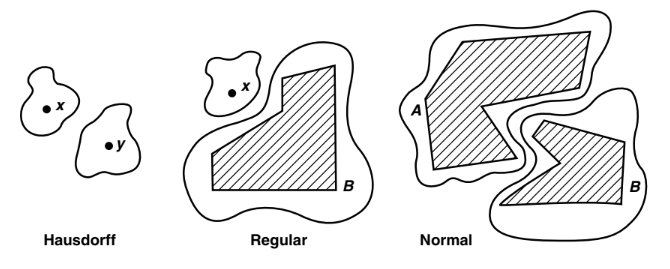
\includegraphics[scale = 0.7]{def4.3}
\centering
\end{figure}

\begin{obs}
Algunas de las propiedades que se tenían en espacios Hausdorff y regulares ahora no son ciertas:
\begin{itemize}
    \item No todo subespacio de un espacio normal es normal.
    \item $X \times Y$ normal $\implies$ $X$ normal e $Y$ normal, pero el recíproco no es cierto.
\end{itemize}
\end{obs}

\begin{proposition}
La normalidad es un invariante topológico.
\end{proposition}

\begin{proof}
Análoga a la de la \hyperref[prop4.3.]{\color{blue}Proposición 4.3}.
\end{proof}

\begin{proposition}
Todo espacio compacto Hausdorff es normal.
\end{proposition}

\begin{proof}
Ejercicio 5 de la Relación 6.
\end{proof}

\begin{theorem}[Caracterización de los espacios normales]
Sea $X$ Hausdorff. Son equivalentes:
\begin{itemize}
    \item[(i)] $X$ es normal.
    \item[(ii)] Dado $F \subset U$ con $F$ cerrado y $U$ abierto, existe otro abierto $V$ tal que $F \subset V \subset \overline{V} \subset U$.
\end{itemize}
\end{theorem}

\begin{proof}
Similar a la del \hyperref[teo4.1.]{\color{blue}Teorema 4.1}.
\end{proof}

En la demostración del próximo teorema, vamos a utilizar lo siguiente: dado un espacio métrico $X$ y dado $A \subset X$...
\begin{itemize}
    \item Si $x \in X$, definimos la \underline{distancia de $x$ a $A$} como
    \[d(x,A) = \inf{\{d(x,y) \mid y \in A\}}\]
    \item $d(x,A) = 0 \iff x \in \overline{A}$.
    \item La aplicación
    \[
    \begin{aligned}[t]
        h_A \colon X & \longrightarrow \R \\
        x & \longmapsto d(x,A)
    \end{aligned}
    \]
    es continua.
\end{itemize}

\begin{theorem}
Todo espacio métrico es normal.
\end{theorem}

\begin{proof}
Sea $X$ espacio métrico y sean $F,G \subset X$ cerrados disjuntos. Definimos
\[\theta_F = \{x \in X \mid d(x,F) < d(x,G)\} \qquad \theta_G = \{x \in X \mid d(x,G) < d(x,F)\}\]
Comprobemos lo necesario:
\begin{itemize}
    \item $F \subset \theta_F$, pues dado $x \in F = \overline{F}$, se tiene que $d(x,F) = 0$, y como $x \notin G = \overline{G}$, entonces $d(x,G) > 0$, luego $d(x,F) < d(x,G)$.
    \item $G \subset \theta_G$ (análogo al punto anterior).
    \item Es claro que $\theta_F \cap \theta_G = \emptyset$.
    \item $\theta_F$ es abierto, pues la aplicación
        \[
        \begin{aligned}[t]
            h_A \colon X & \longrightarrow \R \\
            x & \longmapsto d(x,A)
        \end{aligned}
        \]
    es continua para cualquier $A \subset X$, y tenemos que
    \[\theta_F = (h_G - h_F)^{-1}((0,\infty))\]
    que es abierto por ser la imagen inversa de un abierto mediante una aplicación continua.
    \item $\theta_G$ es abierto (análogo al punto anterior).
\end{itemize}
Por tanto, $X$ es normal.
\end{proof}

\begin{obs}
En general, se tiene que
\[\textrm{Métrico} \overset{(i)}{\Longrightarrow} \textrm{Normal} \overset{(ii)}{\Longrightarrow} \textrm{Regular}\]
\[\textrm{Métrico} \centernot\Longleftarrow \textrm{Normal} \overset{(iii)}{\centernot\Longleftarrow} \textrm{Regular}\]
ya que $(i)$ es cierto por el teorema anterior, $(ii)$ es consecuencia de la \hyperref[prop4.4.]{\color{blue}Proposición 4.4}, y para un ejemplo que demuestre $(iii)$, ver el Ejercicio 8 de la Relación 6.

\vspace{2mm}
Sin embargo, si $X$ es ANII,
\[\textrm{Métrico} \iff \textrm{Normal} \iff \textrm{Regular}\]
\end{obs}

\begin{theorem}[Lema de Urysohn]
Sea $X$ Hausdorff. Son equivalentes:
\begin{itemize}
    \item[(i)] $X$ es normal.
    \item[(ii)] Dados $F,G \subset X$ cerrados disjuntos, existe una aplicación $f \colon X \to [0,1]$ continua con $f(F) = \{0\}, f(G) = \{1\}$.
\end{itemize}
\end{theorem}

\begin{proof}
Veamos primero que $(ii) \implies (i)$. Supongamos que se cumple $(ii)$. Sean $F,G \subset X$ cerrados disjuntos y sea $f \colon X \to [0,1]$ continua tal que $f(F) = \{0\}, f(G) = \{1\}$. Los conjuntos $\theta_F = f^{-1}([0,\frac{1}{2})) \subset F$, $\theta_G = f^{-1}((\frac{1}{2},1]) \subset G$ son abiertos ($f$ es continua y $[0,\frac{1}{2})$, $(\frac{1}{2},1]$ son abiertos de $[0,1]$) y cumplen $\theta_F \cap \theta_G = \emptyset$, luego $X$ es normal.

\vspace{2mm}
Solo vamos a demostrar $(i) \implies (ii)$ para espacios métricos. Sean $F,G$ cerrados disjuntos. Definimos
\[
\begin{aligned}[t]
    f \colon X & \longrightarrow [0,1] \\
    x & \longmapsto \frac{d(x,F)}{d(x,F) + d(x,G)}
\end{aligned}
\]
que es continua por ser cociente de funciones continuas (el denominador nunca se anula) y cumple $f(F) = \{0\}, f(G) = \{1\}$.
\end{proof}

\begin{corollary}
Todo espacio normal conexo de más de un punto tiene cardinal no numerable.
\end{corollary}

\begin{proof}
Sean $x,y \in X$, $x \neq y$. Como los puntos son cerrados, por el lema de Urysohn, existe $f \colon X \to [0,1]$ tal que $f(x) = 0$ y $f(y) = 1$. Como $X$ es conexo, por el teorema de los valores intermedios, dado $t \in [0,1]$, existe $x_t \in X$ tal que $f(x_t) = t$, luego $\mathcal{X}(X) > \mathcal{X}_0$.
\end{proof}

\begin{theorem}[Teorema de extensión de Tietze]
Sea $X$ Hausdorff. Son equivalentes:
\begin{itemize}
    \item[(i)] $X$ es normal.
    \item[(ii)] Dado $A \subset X$ cerrado y $f \colon A \to \R$ continua, existe $\tilde{f} \colon X \to \R$ continua con $\bigl.\tilde{f}\bigr|_A = f$.
\end{itemize}
\end{theorem}

\begin{proof}
Solo vamos a demostrar $(ii) \implies (i)$. Supongamos que se cumple $(ii)$. Sean $F,G$ cerrados disjuntos. Tomemos $A = F \cup G$. Definimos $f \colon A \to \R$ por
\[
f(x) = 
\begin{cases}
0 & $si$ \ x \in F \\
1 & $si$ \ x \in G
\end{cases}
\]
que es continua (\hyperref[prop1.16.]{\color{blue}Proposición 1.16}). Por $(ii)$, existe $\tilde{f} \colon X \to \R$ continua con $\bigl.\tilde{f}\bigr|_A = f$. Sean 
\[\theta_F = \tilde{f}^{-1}((-\infty,\frac{1}{2})) \supset F \qquad \theta_G = \tilde{f}^{-1}((\frac{1}{2},\infty)) \supset G\]
Entonces $\theta_F \cap \theta_G = \emptyset$, luego $X$ es normal.
\end{proof}

\end{document}
